% Opcje klasy 'iithesis' opisane sa w komentarzach w pliku klasy. Za ich pomoca
% ustawia sie przede wszystkim jezyk oraz rodzaj (lic/inz/mgr) pracy.
\documentclass[shortabstract]{iithesis}

\usepackage[utf8]{inputenc}

%%%%% DANE DO STRONY TYTUŁOWEJ
% Niezaleznie od jezyka pracy wybranego w opcjach klasy, tytuł i streszczenie
% pracy nalezy podac zarowno w jezyku polskim, jak i angielskim.
% Pamietaj o madrym (zgodnym z logicznym rozbiorem zdania oraz estetyka) recznym
% złamaniu wierszy w temacie pracy, zwlaszcza tego w jezyku pracy. Uzyj do tego
% polecenia \fmlinebreak.
\polishtitle    {Aplikacja webowa do obsługi\fmlinebreak rozgrywek tenisowych}
\englishtitle   {Web application for managing tennis tournaments}
\polishabstract {Celem pracy jest zaprojektowanie i stworzenie aplikacji webowej umożliwiającej organizację rozgrywek tenisa ziemnego. Projekt obejmuje opracowanie responsywnego interfejsu użytkownika wraz z zapleczem. Każdy element aplikacji został skonteneryzowany i skonfigurowany do współpracy z resztą projektu.}
\englishabstract{The aim of this work is to design and create web application for organizing tennis tournaments. The project includes developing responsive user interface along with the backend. Each component of the application has been contenerized and configured to work with the rest of the project.}
% w pracach wielu autorow nazwiska mozna oddzielic poleceniem \and
\author         {Marcin Wróbel}
% w przypadku kilku promotorow, lub koniecznosci podania ich afiliacji, linie
% w ponizszym poleceniu mozna zlamac poleceniem \fmlinebreak
\advisor        {dr hab. Dariusz Biernacki}
%\date          {}                     % Data zlozenia pracy
% Dane do oswiadczenia o autorskim wykonaniu
\transcriptnum {323830}                     % Numer indeksu
\advisorgen    {dr hab. Dariusza Biernackiego} % Nazwisko promotora w dopelniaczu
%%%%%

%%%%% WŁASNE DODATKOWE PAKIETY
%
\usepackage{float,dirtree,subfig,enumitem}
\usepackage[export]{adjustbox}
% \usepackage{graphicx,listings,amsmath,amssymb,amsthm,amsfonts,tikz}
\usepackage{graphicx,listings,amsmath}
%
%%%%% WŁASNE DEFINICJE I POLECENIA
%
%\theoremstyle{definition} \newtheorem{definition}{Definition}[chapter]
%\theoremstyle{remark} \newtheorem{remark}[definition]{Observation}
%\theoremstyle{plain} \newtheorem{theorem}[definition]{Theorem}
%\theoremstyle{plain} \newtheorem{lemma}[definition]{Lemma}
%\renewcommand \qedsymbol {\ensuremath{\square}}
% ...
\usepackage{listings}
\lstset{
  literate={ą}{{\k a}}1
           {Ą}{{\k A}}1
           {ż}{{\. z}}1
           {Ż}{{\. Z}}1
           {ź}{{\' z}}1
           {Ź}{{\' Z}}1
           {ć}{{\' c}}1
           {Ć}{{\' C}}1
           {ę}{{\k e}}1
           {Ę}{{\k E}}1
           {ó}{{\' o}}1
           {Ó}{{\' O}}1
           {ń}{{\' n}}1
           {Ń}{{\' N}}1
           {ś}{{\' s}}1
           {Ś}{{\' S}}1
           {ł}{{\l}}1
           {Ł}{{\L}}1
}
\usepackage{sourcecodepro}
\usepackage[T1]{fontenc}
\lstset{basicstyle=\ttfamily}
%%%%%

\begin{document}

%%%%% POCZĄ„TEK ZASADNICZEGO TEKSTU PRACY

\chapter{Wprowadzenie}
Obsługa amatorskich lig tenisa ziemnego bardzo często polega na wykorzystaniu notesu i długopisu.
W ramach tych lig zawodnicy są zazwyczaj zobowiązani do własnej organizacji meczów i pozyskiwania danych kontaktowych innych uczestników w celu ustalenia terminów spotkań.
Pojawiła się potrzeba stworzenia nowoczesnego narzędzia do organizacji amatorskich rozgrywek ligowych.
W poniższej pracy przedstawiono aplikację webową, która odpowiada na tę potrzebę.
\par
Aplikacja umożliwia łatwe wprowadzanie wyników meczów, weryfikuje je oraz uwzględnia przypadki szczególne, takie jak walkover, czy krecz.
Na podstawie wyników meczów sytuacja w grupie i drabince turniejowej jest obliczana automatycznie.
Zawodnicy mają dostęp do danych kontaktowych osób, z którymi mają rozegrać mecz. Są również powiadamiani o zakończonych meczach i zmianach w tabeli.
Aplikacja udostępnia także bogatą parametryzację, pozwalającą dostosować system do wymagań danej rozgrywki.
\par
Aplikacja została stworzona z wykorzystaniem nowoczesnych i popularnych technologii.
Warstwa frontendowa została napisana z użyciem frameworka Vue.js, który pozwala na tworzenie dynamicznego interfesju użytkownika z komponentami wielokrotnego użytku.
Z kolei backend został napisany w frameworku Spring Boot, który zapewnia niezawodność i wydajność.
Dane, niezbędne do sprawnego funkcjonowania aplikacji, są przechowywane w bazie danych PostgreSQL.
Całość została skonteneryzowana za pomocą technologii Docker.
\par
Co istotne, dzięki responsywnemu interfejsowi użytkownika, aplikacja jest przystosowana zarówno do urządzeń mobilnych, jak i~stacjonarnych.
Dzięki temu zawodnicy mają możliwość korzystania z systemu nie tylko w domu, ale również w~przerwach w pracy, czy na korcie tenisowym.
Aplikacja webowa została opublikowana i~jest dostępna na stronie \texttt{www.rozgrywkitenisa.pl}.
\par

\chapter{Specyfikacja zagadnienia}
W tym rozdziale zostanie opisana specyfikacja projektu będącego przedmiotem niniejszej pracy.
Specyfikacja obejmuje opis funkcjonalności, algorytmy odpowiadające za organizację rozgrywki, oraz przypadki użycia.
\section{Funkcjonalności}
\noindent
Poniżej przedstawiono listę funkcjonalności zrealizowanych w ramach pracy:
\begin{itemize}
    \item Aplikacja umożliwia tworzenie rozgrywek. Rozgrywka może być dwuczęściowa: na początku zawodnicy rywalizują w fazie grupowej, a następnie najlepsi awansują do fazy pucharowej.
          Rozgrywka może być też jednoczęściowa: faza grupowa jest pominięta i wszyscy zawodnicy zaczynają od fazy pucharowej.
    \item Liczba grup i zawodników w fazie pucharowej jest konfigurowalna.
          W pojedynczej rozgrywce liczba zawodników została ograniczona do 128, a liczba grup została ograniczona do 24.
          Limity zostały wybrane arbitralnie i mogą zostać zmienione.
          Niestety, limity są konieczne, ponieważ nie można pozwolić użytkownikowi na stworzenie rozgrywki o bardzo dużej (np. 10000) liczbie grup lub zawodników.
          Przeglądarka nie potrafiłaby ich wyrenderować.
    \item Podczas tworzenia rozgrywki skład grup jest losowany. Losowanie jest wspomagane rankingiem.
          W przypadku rozgrywek bez fazy grupowej rozstawienie zawodników w fazie pucharowej ustalane jest na podstawie rankingu.
    \item Zawodnicy mają dostęp do danych kontaktowych osób, z którymi będą rozgrywać mecz.
    \item Wynik meczu może wpisywać organizator/sędzia lub zawodnicy.
    \item Wynik meczu powinien obsługiwać przypadki szczególne:
          \begin{itemize}
              \item walkower - w tabeli wynik liczony jest tak, jakby zawodnik poddający się przegrał wszystkie gemy, aż do zwycięstwa w~meczu drugiego zawodnika,
              \item krecz - w tabeli wynik liczony jest tak, jakby zawodnik poddający się przegrał wszystkie gemy od momentu wycofania się, aż do zwycięstwa w~meczu drugiego zawodnika.
          \end{itemize}
    \item Aplikacja obsługuje rejestrację i logowanie użytkowników. Każdy użytkownik może zresetować swoje hasło za pomocą emaila podanego podczas rejestracji.
    \item Aplikacja oblicza ranking zawodników na podstawie zakończonych rozgrywek.
\end{itemize}
\section{Generowanie grup}
Podczas generowania grup zawodnicy są dzieleni na koszyki według rankingu.
Dla rozgrywki o $N$ zawodnikach i $M$ grupach w pierwszym koszyku znajduje się $M$ zawodników o najlepszym rankingu, w drugim koszyku kolejne $M$ zawodników, itd.
Wyjątkiem jest ostatni koszyk. Jeżeli $N \not\equiv 0 \pmod{M}$, wtedy liczba zawodników w~ostatnim koszyku jest mniejsza, wynosi $N\bmod{M}$.
\section{Generowanie drabinki fazy pucharowej}
Na początku generowania drabinki fazy pucharowej wszyscy zawodnicy biorący udział w rozgrywce są sortowani.
Jeżeli rozgrywka posiada fazę grupową, to kolejność zależy od wyników w grupie.
Największe znaczenie ma pozycja w grupie, potem bilans meczów, bilans setów, a na końcu bilans gemów.
Jeżeli rozgrywka składa się tylko z fazy pucharowej, to kolejność zawodników zależy od pozycji w rankingu ogólnym.

Posortowanym zawodnikom przypisane zostają numery startowe od $0$ do $N-1$, gdzie $N$ to liczba zawodników.
Numery startowe są następnie przypisywane do drabinki według poniższego algorytmu. Jego wizualizacja znajduje się na rysunku~\ref{fig:knockout_bracket_generation}.
\begin{lstlisting}
    numeryStartowe=[0,1]
    dopóki (numeryStartowe.rozmiar() < N) {
        poprzednieNumeryStartowe = numeryStartowe
        numeryStartowe = []
        największyNumer = poprzednieNumeryStartowe.rozmiar() * 2 - 1
        dla każdego (ns w poprzednieNumeryStartowe) {
            numeryStartowe.dodaj(ns)
            numeryStartowe.dodaj(największyNumer - ns)
        }
    }
    zwróć numeryStartowe
\end{lstlisting}
Kolejne pary w zwróconej liście odpowiadają kolejnym parom w drabince fazy pucharowej.
Przykładowo dla $N=8$ zostanie zwrócona lista $[0, 7, 3, 4, 1, 6, 2, 5]$. Odpowiada to parom
$[0, 7]$, $[3, 4]$, $[1, 6]$, $[2, 5]$.
\begin{figure}[H]
    \centering
    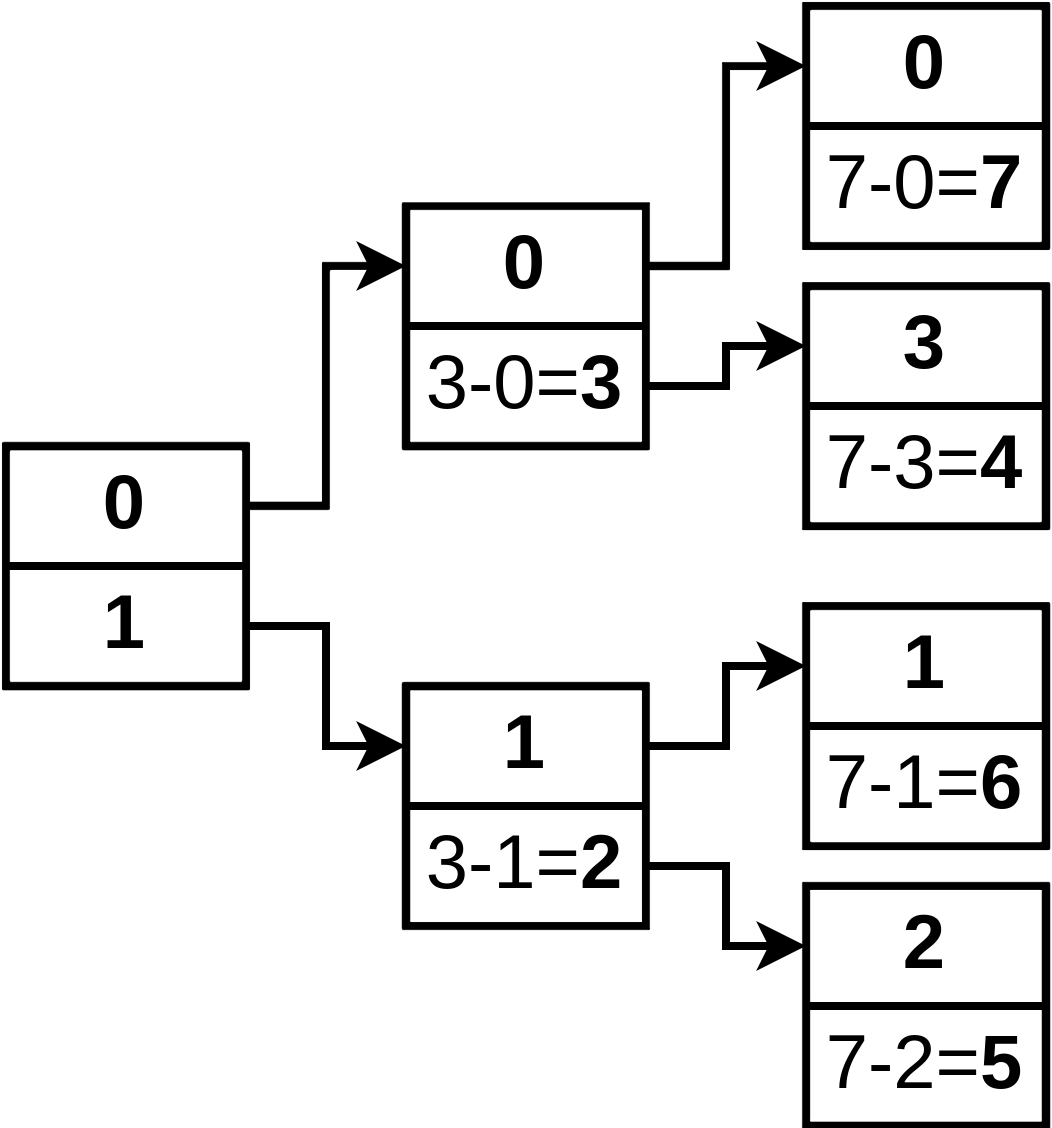
\includegraphics[width=0.5\textwidth]{assets/generowanie_drabinki.png}
    \caption{Schemat generowania drabinki fazy pucharowej}
    \label{fig:knockout_bracket_generation}
\end{figure}
\section{Obliczanie rankingu}
Do obliczania rankingu brane są pod uwagę tylko ukończone rozgrywki.
Ukończona rozgrywka to taka rozgrywka, w której mecz finałowy ma wpisany wynik.
Punkty do rankingu dodawane są według punktacji zdefiniowanej dla każdej rozgrywki.
Wyświetlana w aplikacji lista rankingowa wyświetla także względną zmianę pozycji dla każdego zawodnika.
Zmiana pozycji obliczana jest poprzez porównanie aktualnej pozycji zawodnika z jego pozycją przed zakończeniem ostatniej rozgrywki.



\section{Przypadki użycia}
W tej sekcji zostaną opisane przypadki użycia aplikacji webowej, będącej przedmiotem tej pracy.
Ich celem jest zademonstrowanie działania programu.
\subsection{Tworzenie nowej rozgrywki}
\begin{tabular}{|l|p{12cm}|}
    \hline
    Nazwa      & Tworzenie nowej rozgrywki                                                                                                                                                               \\
    \hline
    Aktor      & Organizator rozgrywki                                                                                                                                                                   \\
    \hline
    Scenariusz &
    \begin{enumerate}[nosep,leftmargin=*,rightmargin=8pt,before=\vspace{-7.5pt},after=\vspace{-8pt}]
        \item Użytkownik znajduje się na stronie rozgrywek i klika przycisk ``Utwórz rozgrywkę''.
        \item Użytkownik uzupełnia wszystkie pola konfiguracyjne: nazwę, czas trwania, liczbę zawodników, liczbę grup, liczbę finalistów, liczbę setów do wygranej, punkty do zdobycia za poszczególne etapy.
        \item Użytkownik wyszukuje zawodników używając pola wyszukiwania i~wybiera ich poprzez kliknięcie.
        \item Użytkownik klika przycisk ``Wylosuj skład grup'' i aplikacja losuje skład grup.
        \item Użytkownik klika przycisk ``Utwórz'', aplikacja tworzy rozgrywkę i~przekierowuje użytkownika do strony z nowo utworzoną rozgrywką.
    \end{enumerate} \\
    \hline
\end{tabular}

\subsection{Dodawanie wyniku meczu}
\begin{tabular}{|l|p{12cm}|}
    \hline
    Nazwa                                                     & Dodawanie wyniku meczu                                               \\
    \hline
    Aktor                                                     & Zawodnik meczu, który się zakończył                                  \\
    \hline
    Scenariusz                                                &
    \begin{enumerate}[nosep,leftmargin=*,rightmargin=8pt,before=\vspace{-7.5pt},after=\vspace{-8pt}]
        \item Użytkownik znajduje się na stronie rozgrywek i wpisuje w polu wyszukiwania nazwę rozgrywki w ramach, której odbył się mecz.
        \item Użytkownik klika rozgrywkę, którą wyświetliła mu aplikacja.
        \item Użytkownik klika grupę, w której się znajduje.
        \item Użytkownik klika mecz, którego wynik chce dodać.
        \item Użytkownik klika ikonę edycji i wprowadza wynik meczu.
        \item Użytkownik zatwierdza wynik meczu klikając ikonę zapisu.
        \item Aplikacja wysyła email do wszystkich zawodników w grupie informując o nowym wyniku.
    \end{enumerate} \\
    \hline
    \vtop{\hbox{\strut Scenariusz}\hbox{\strut alternatywny}} &
    \begin{enumerate}[nosep,leftmargin=19.5pt,rightmargin=8pt,before=\vspace{-7.5pt},after=\vspace{-8pt}]
        \item [6a.] Użytkownik klika na ikonę walkowera, aby ustawić wynik meczu jako walkower.
        \item [7a.] Użytkownik zatwierdza wynik meczu klikając ikonę zapisu.
        \item [8a.] Aplikacja wysyła email do wszystkich zawodników w grupie informując o nowym wyniku.
    \end{enumerate}               \\
    \hline
\end{tabular}

\subsection{Podgląd danych kontaktowych zawodników w grupie}
\begin{tabular}{|l|p{12cm}|}
    \hline
    Nazwa                                                      & Podgląd danych kontaktowych zawodników w grupie         \\
    \hline
    Aktor                                                      & Zawodnik biorący udział w rozgrywce                     \\
    \hline
    Scenariusz                                                 &
    \begin{enumerate}[nosep,leftmargin=*,rightmargin=8pt,before=\vspace{-7.5pt},after=\vspace{-8pt}]
        \item Użytkownik wchodzi na stronę logowania.
        \item Użytkownik loguje się podając nazwę użytkownika lub email oraz hasło.
        \item Użytkownik wchodzi na stronę z listą rozgrywek i klika rozgrywkę w której bierze udział.
        \item Użytkownik klika ``Pokaż dane kontaktowe'' i~system je wyświetla.
    \end{enumerate}      \\
    \hline
    \vtop{\hbox{\strut Scenariusze}\hbox{\strut alternatywne}} &
    \begin{enumerate}[nosep,leftmargin=19.5pt,rightmargin=8pt,before=\vspace{-7.5pt},after=\vspace{-8pt}]
        \item [2a.] Użytkownik loguje się podając nazwę użytkownika lub email oraz niepoprawne hasło.
        \item [3a.] System wyświetla komunikat ``Niepoprawna nazwa użytkownika lub hasło''.
    \end{enumerate} \\
    \cline{2-2}
                                                               &
    \begin{enumerate}[nosep,leftmargin=19.5pt,rightmargin=8pt,before=\vspace{-7.5pt},after=\vspace{-8pt}]
        \item [3b.] Użytkownik wchodzi na stronę z listą rozgrywek i klika rozgrywkę w której nie bierze udziału.
        \item [4b.] Użytkownik klika ``Pokaż dane kontaktowe'' i~system nie wyświetla danych kontaktowych nikogo.
    \end{enumerate} \\
    \hline
\end{tabular}

\chapter{Opis aplikacji}
Ten rozdział zaczyna się od opisu interfejsu aplikacji pozwalając użytkownikowi zapoznać się z nim.
Następnie znajduje się porównanie aplikacji z innymi znanymi rozwiązaniami.
Na końcu przedstawione zostały kroki pozwalające na instalację aplikacji lokalnie lub w środowisku produkcyjnym.
\section{Interfejs użytkownika}
W tej sekcji zostaną omówione elementy interfejsu użytkownika wraz z zrzutami ekranu pokazującymi wygląd aplikacji na urządzeniach stacjonarnych i mobilnych.
Jeżeli podany został tylko zrzut ekranu w wersji dla komputerów, oznacza to, że wersja mobilna niewiele się różni.
\subsection{Pasek nawigacyjny}
Pasek nawigacyjny~(\ref{fig:navigation_bar}) ułatwia poruszanie się po stronie. Logo (piłka tenisowa) z lewej strony przekierowuje na stronę główną.
Następne trzy elementy: ``Home'', ``Rozgrywki'' i ``Ranking'' przenoszą odpowiednio na stronę główną, do widoku z listą rozgrywek i do widoku z listą rankingową.
Z prawej strony znajduje się nazwa użytkownika, jeżeli użytkownik jest zalogowany, i przycisk do wylogowywania się.
Dla niezalogowanych użytkowników widoczne są przyciski przenoszące na stronę logowania oraz rejestracji.
Na końcu znajduje się ikona konta pozwalająca zobaczyć status konta. Wersja mobilna wygląda podobnie.
Dodane zostały ikony opisujące linki. Linki rozwijają się i chowają po naciśnięciu przycisku menu w lewym górnym rogu.

\newpage
\begin{figure}[H]
    \centering
    \subfloat[Wersja na komputery]{
        
\includegraphics[width=\textwidth,valign=t]{assets/interfejs/navbar_desktop.png}
    }
    \hfill
    \subfloat[Wersja na telefony]{
        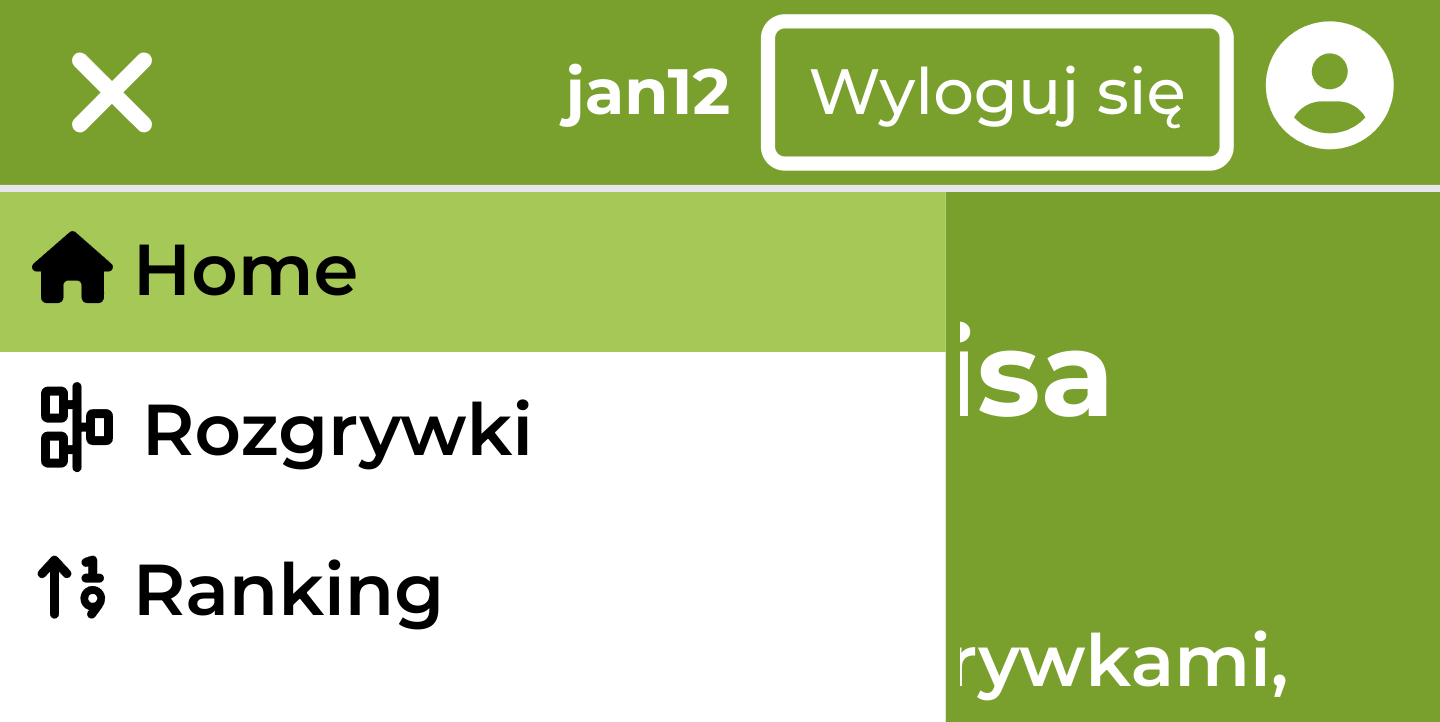
\includegraphics[width=0.5\textwidth,valign=t]{assets/interfejs/navbar_mobile.png}
    }
    \caption{Pasek nawigacyjny}
    \label{fig:navigation_bar}
\end{figure}

\subsection{Widok strony głównej}
Strona główna~\ref{fig:view_home_page} dostarcza użytkownikowi ogólne informacje o tym, co oferuje aplikacja webowa oraz umożliwia przejście do różnych części projektu poprzez linki w pasku nawigacyjnym i wyeksponowane przyciski.

\begin{figure}[H]
    \centering
    \subfloat[Wersja na komputery]{
        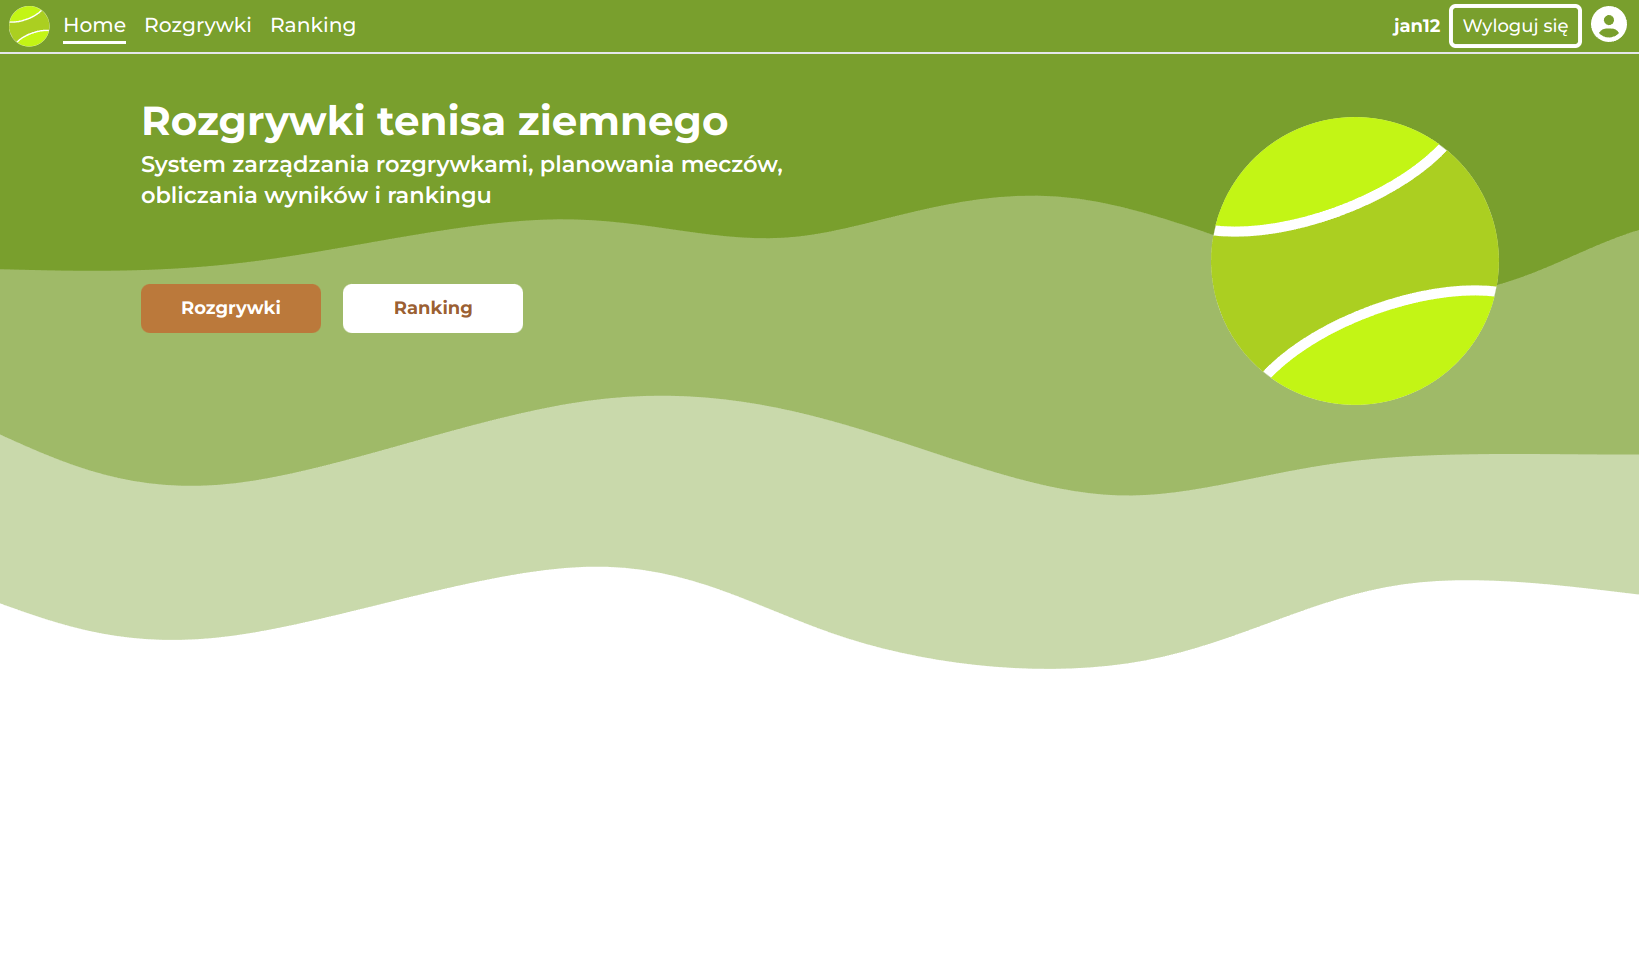
\includegraphics[width=0.72\textwidth,valign=t]{assets/interfejs/home_desktop.png}
        \vphantom{
\includegraphics[width=0.22\textwidth,valign=t]{assets/interfejs/home_mobile.png}}
    }
    \hfill
    \subfloat[Wersja na telefony]{
        
\includegraphics[width=0.22\textwidth,valign=t]{assets/interfejs/home_mobile.png}
    }
    \caption{Strona główna}
    \label{fig:view_home_page}
\end{figure}

\subsection{Widok logowania i rejestracji}
Widoki logowania i rejestracji~(\ref{fig:view_login_and_registration}) są do siebie bardzo podobne.
Strona rejestracji pozwala na stworzenie konta. Nowe konta nie mają uprawnień do organizowania turnieju.
W celu uzyskania uprawnień administrator musi nadać odpowiednie uprawnienia użytkownikowi.
\begin{figure}[H]
    \centering
    \subfloat[Widok rejestracji]{
        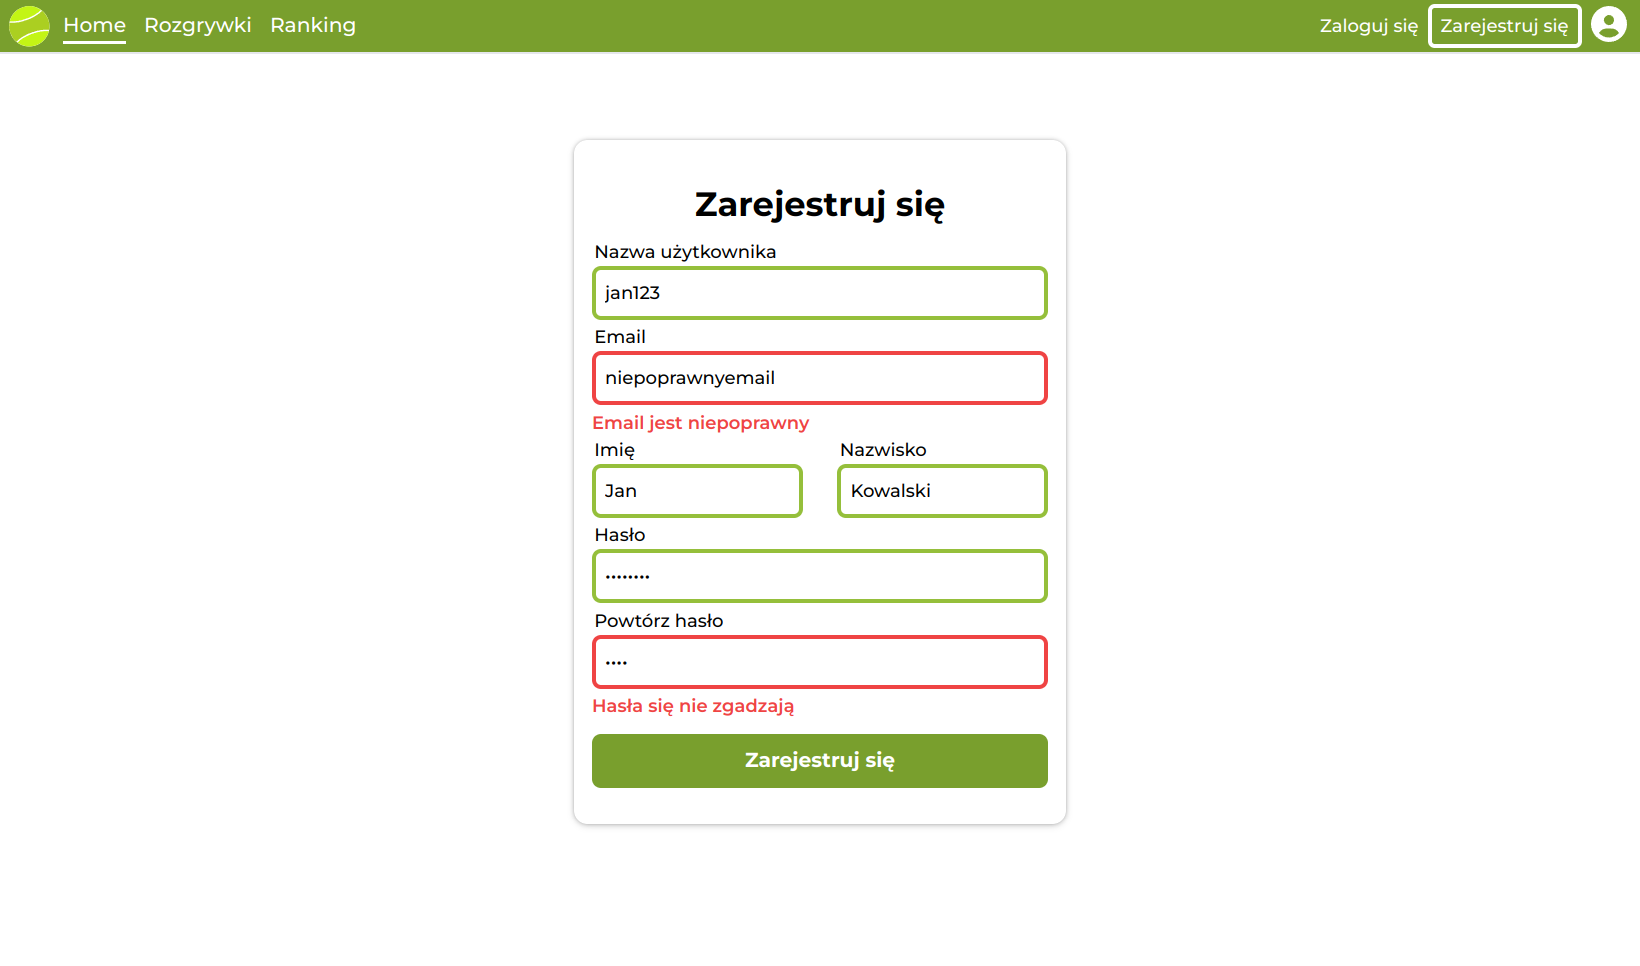
\includegraphics[width=0.44\textwidth,valign=t]{assets/interfejs/rejestracja_desktop.png}
    }
    \hfill
    \subfloat[Widok logowania]{
        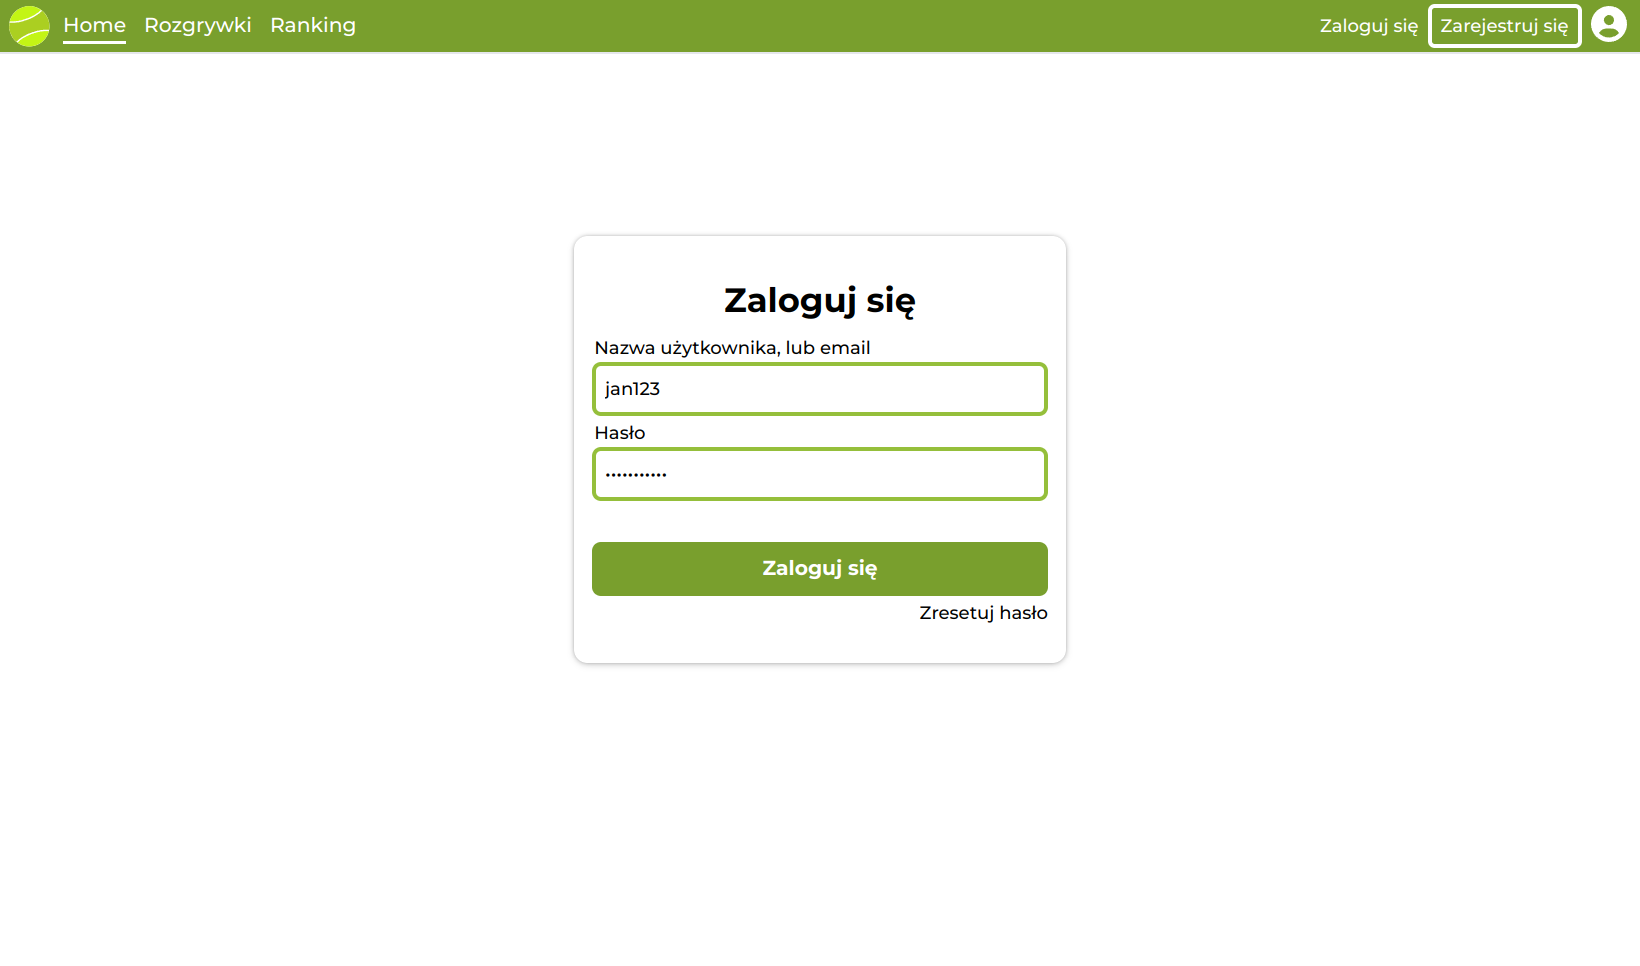
\includegraphics[width=0.44\textwidth,valign=t]{assets/interfejs/logowanie_desktop.png}

    }
    \caption{Widoki logowania i rejestracji}
    \label{fig:view_login_and_registration}
\end{figure}
\subsection{Widok listy rozgrywek}
Widok rozgrywek~(\ref{fig:view_tournaments}) zawiera listę rozgrywek oraz pozwala na wyszukiwanie konkretnej rozgrywki po nazwie.
Każda rozgrywka jest opisana podstawowymi informacjami, a po kliknięciu użytkownik jest przenoszony na stronę ze szczegółami.
Dodatkowo strona zawiera przycisk "Utwórz rozgrywkę" przenoszący do widoku tworzenia rozgrywki.


\begin{figure}[H]
    \centering
    \subfloat[Wersja na komputery]{
        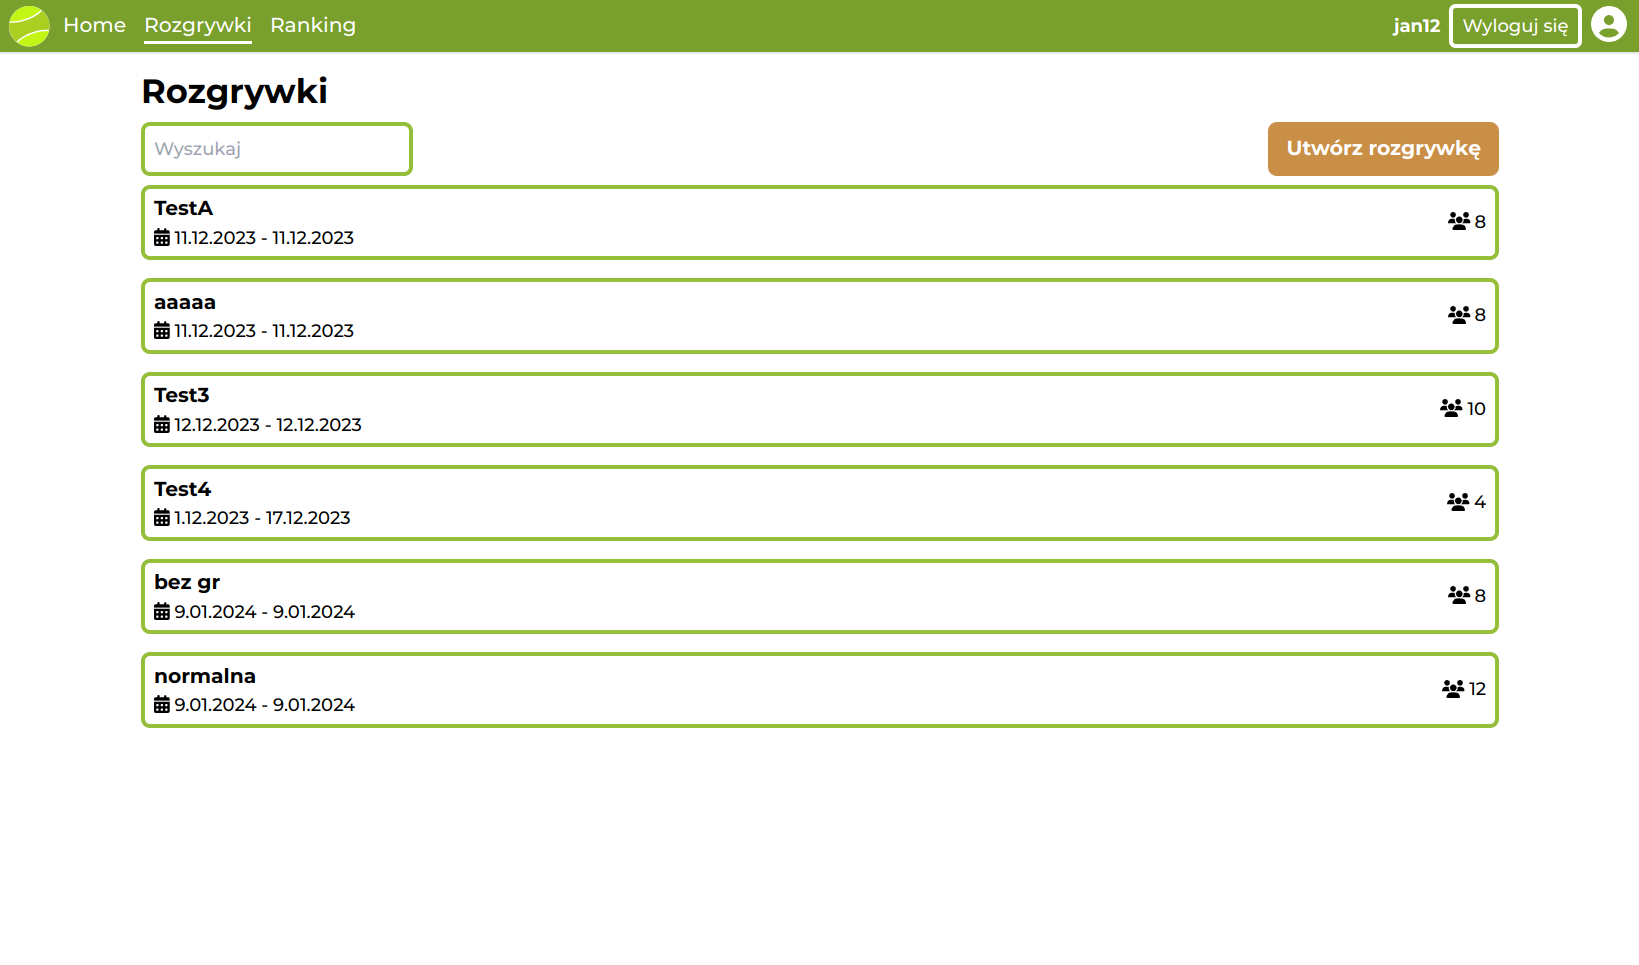
\includegraphics[width=0.72\textwidth,valign=t]{assets/interfejs/rozgrywki_desktop.png}
        \vphantom{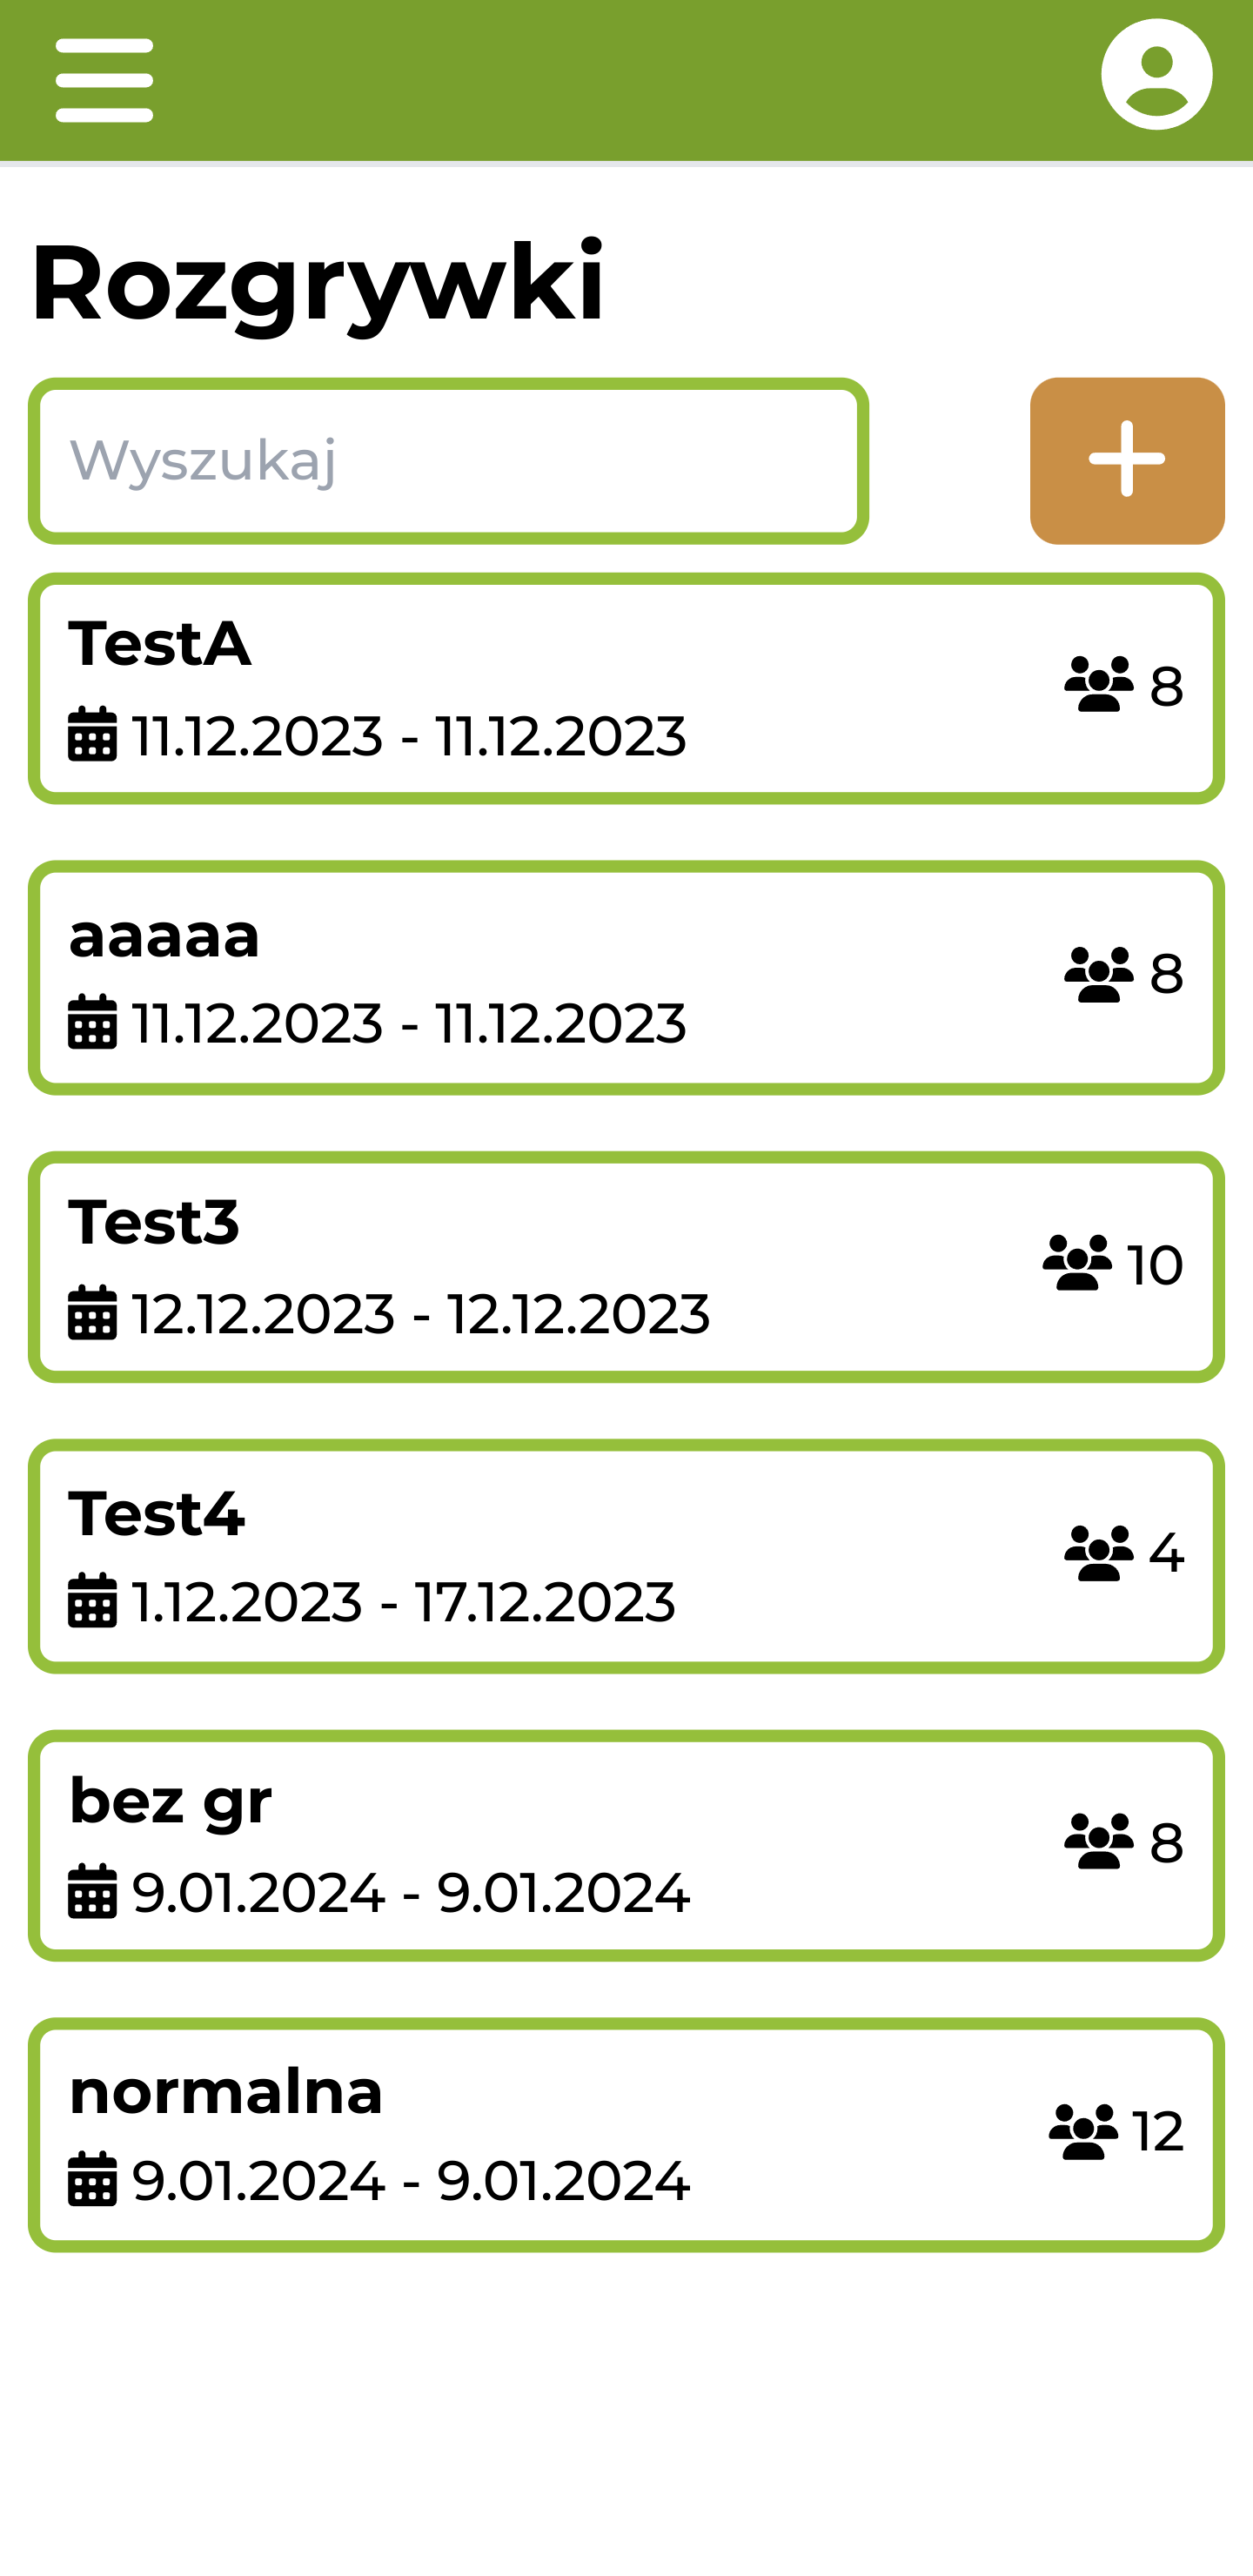
\includegraphics[width=0.22\textwidth,valign=t]{assets/interfejs/rozgrywki_mobile.png}}
    }
    \hfill
    \subfloat[Wersja na telefony]{
        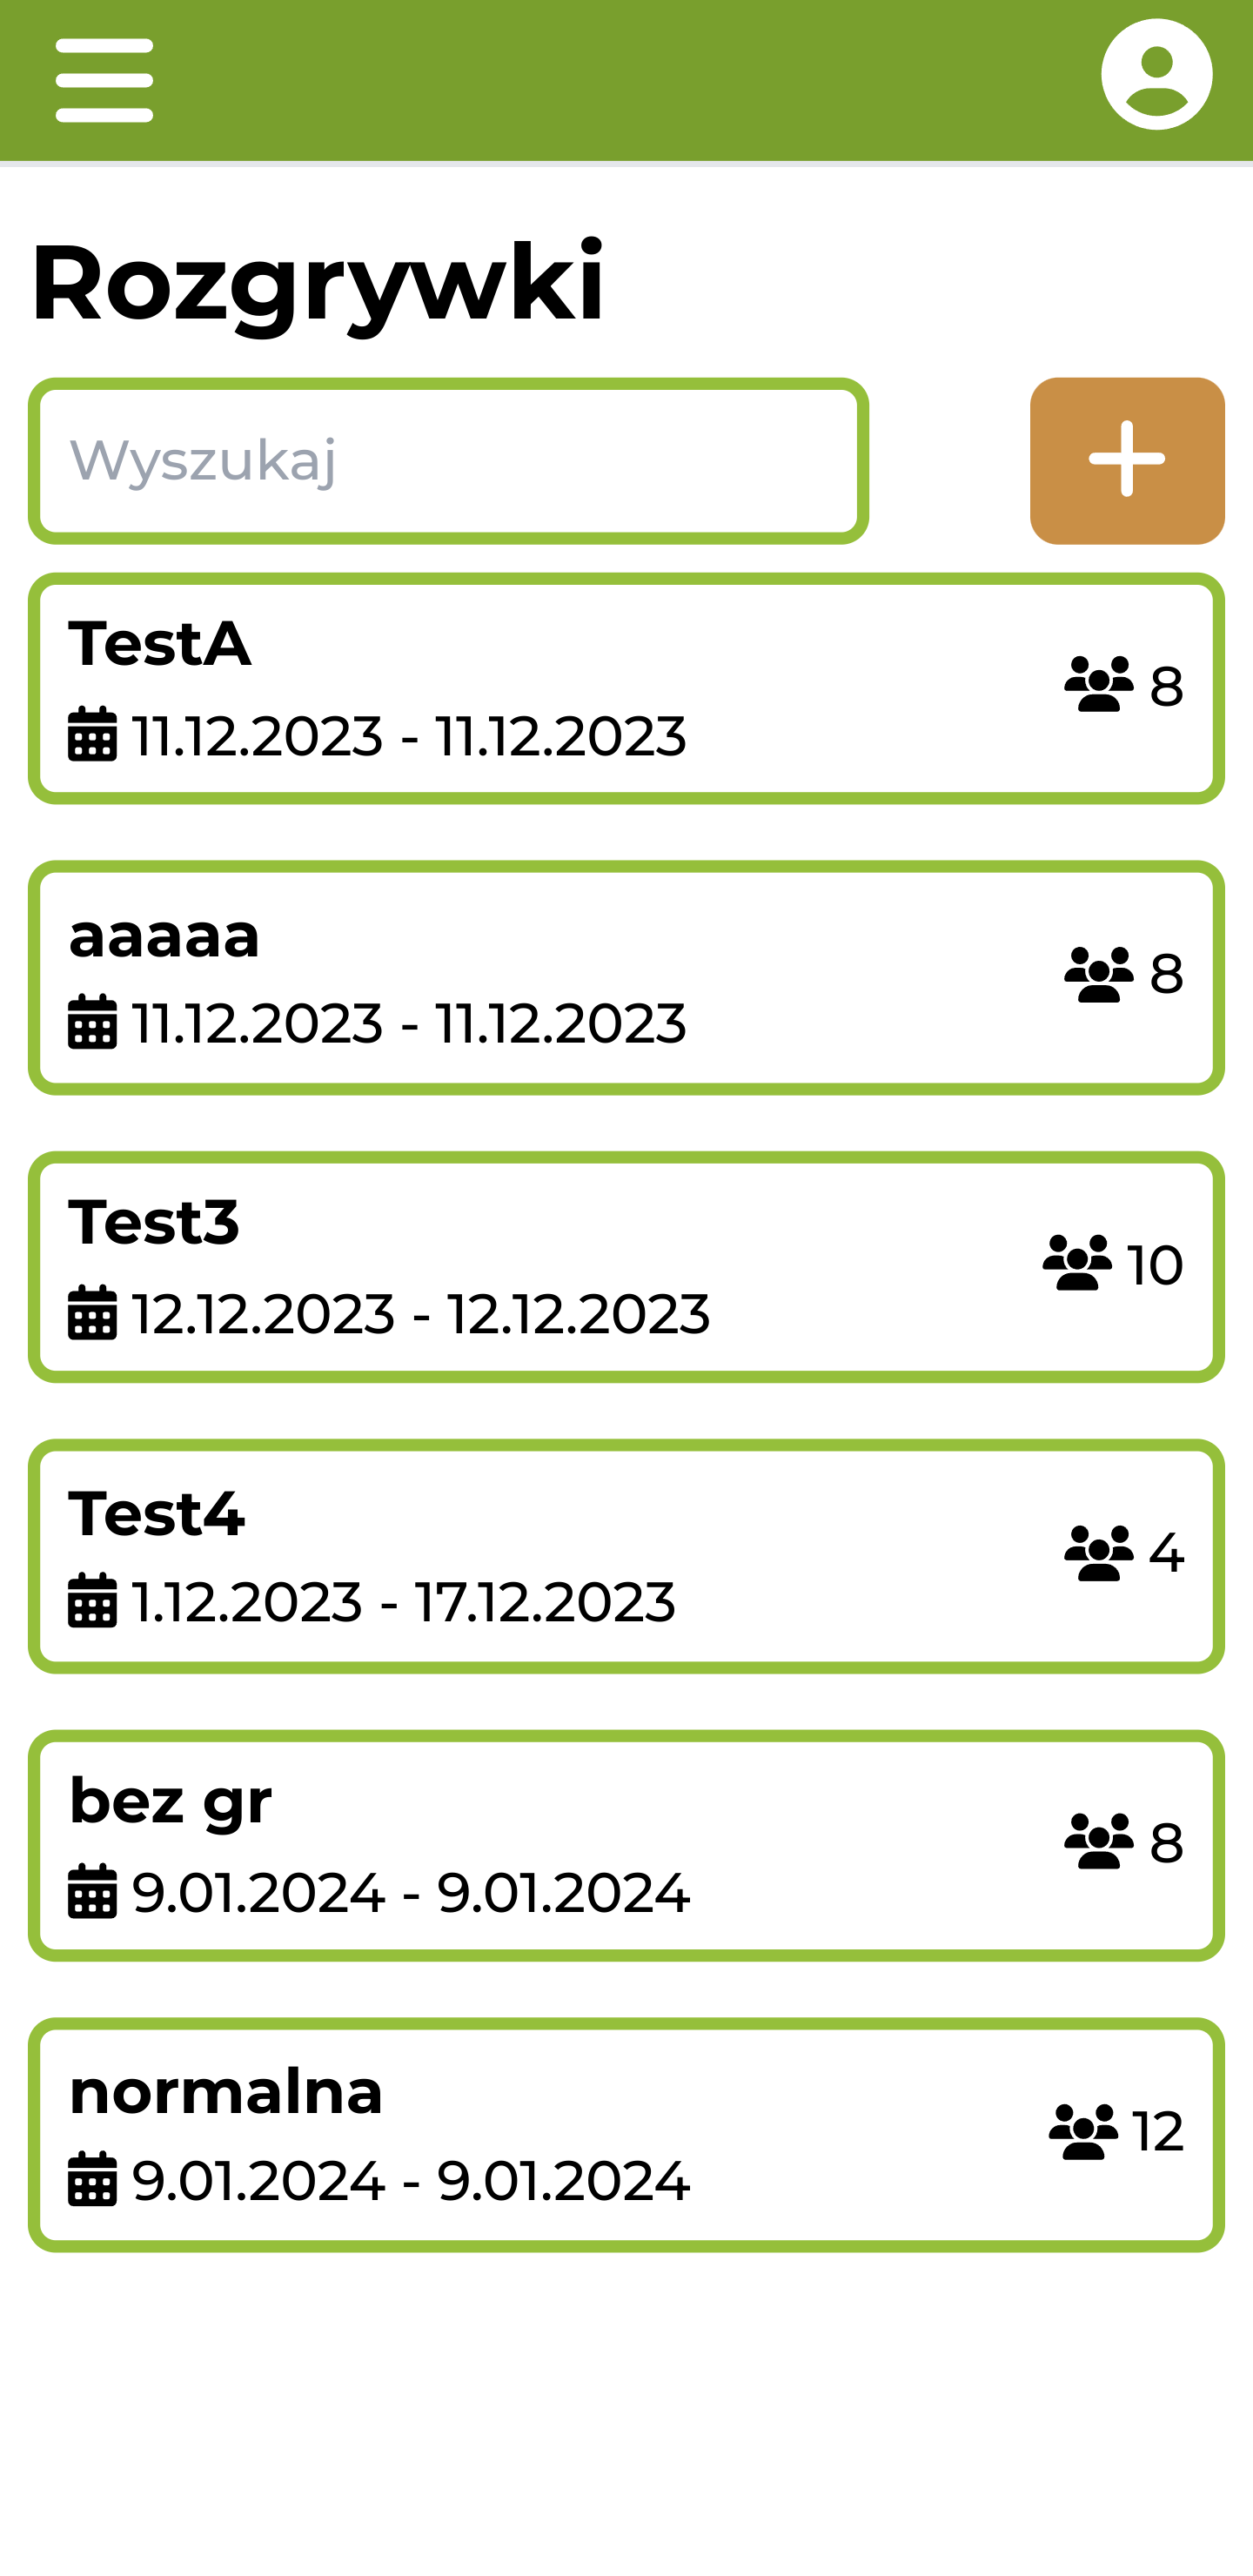
\includegraphics[width=0.22\textwidth,valign=t]{assets/interfejs/rozgrywki_mobile.png}
    }
    \caption{Strona rozgrywek}
    \label{fig:view_tournaments}
\end{figure}

\newpage
\subsection{Widok tworzenia rozgrywki}
Dostęp do tego widoku~(\ref{fig:view_create_tournament}) mają tylko zalogowani użytkownicy z uprawnieniami do tworzenia rozgrywek.
Użytkownik może dostosować wszystkie widoczne parametry. Dostępne opcje parametru \texttt{liczba finalistów}, są zależne od \texttt{liczby zawodników}.
\texttt{Liczba finalistów} musi być potęgą dwójki i nie może być większa od \texttt{liczby zawodników}.
Pole wyszukiwania zawodników pozwala na dodanie ich rozgrywki, a przycisk ``Wylosuj skład grup'' tworzy grupy zgodnie z podziałem na koszyki.

\begin{figure}[H]
    \centering
    \subfloat[Wersja na komputery]{
        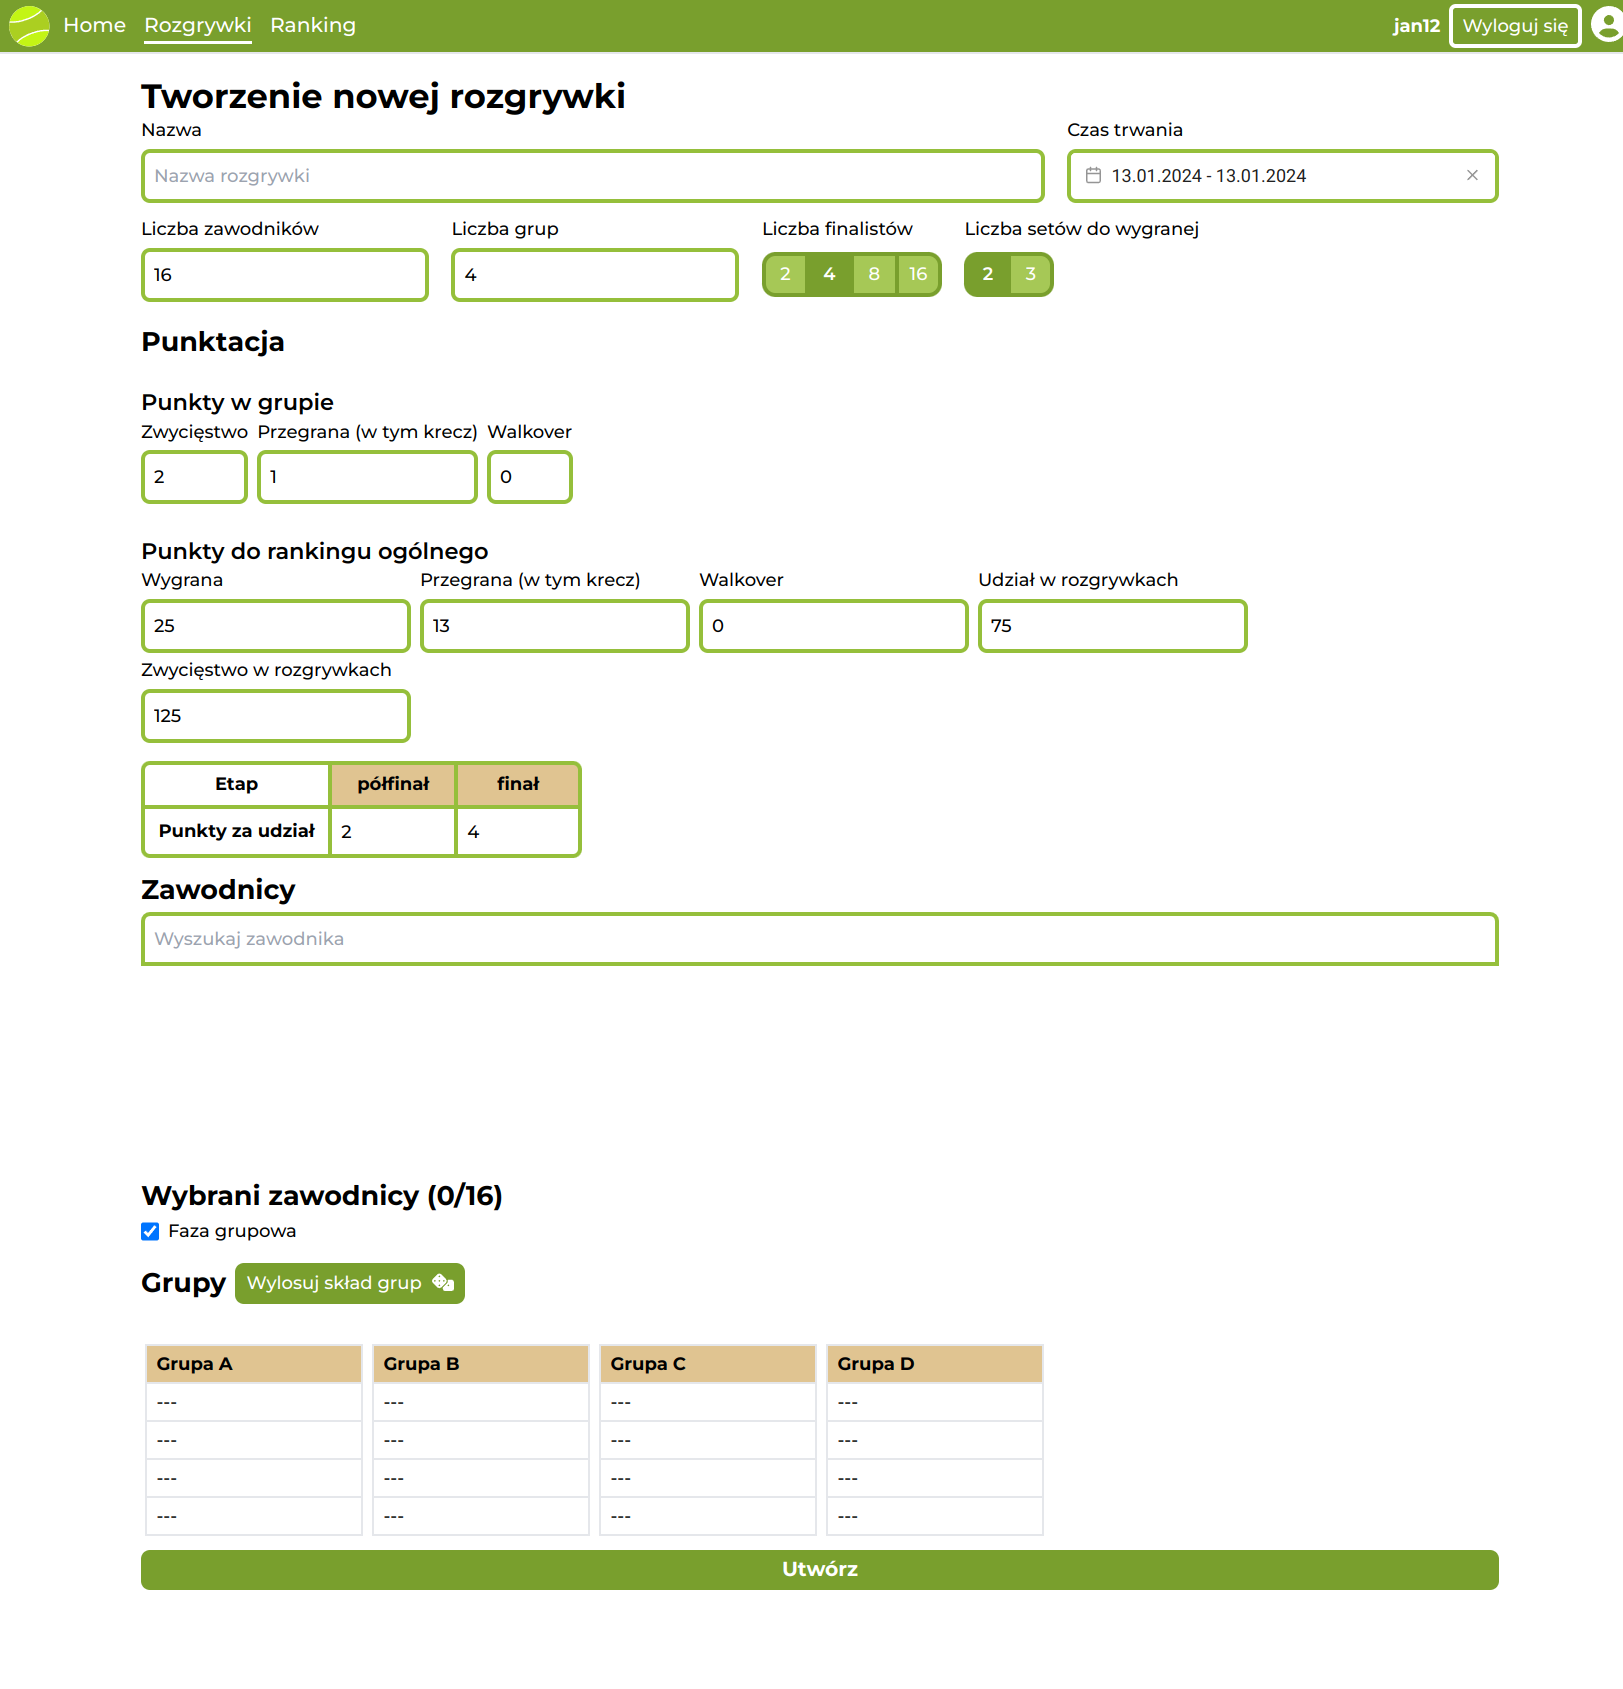
\includegraphics[width=0.72\textwidth,valign=t]{assets/interfejs/rozgrywki_utworz_desktop.png}
    }
    \hfill
    \subfloat[Wersja na telefony]{
        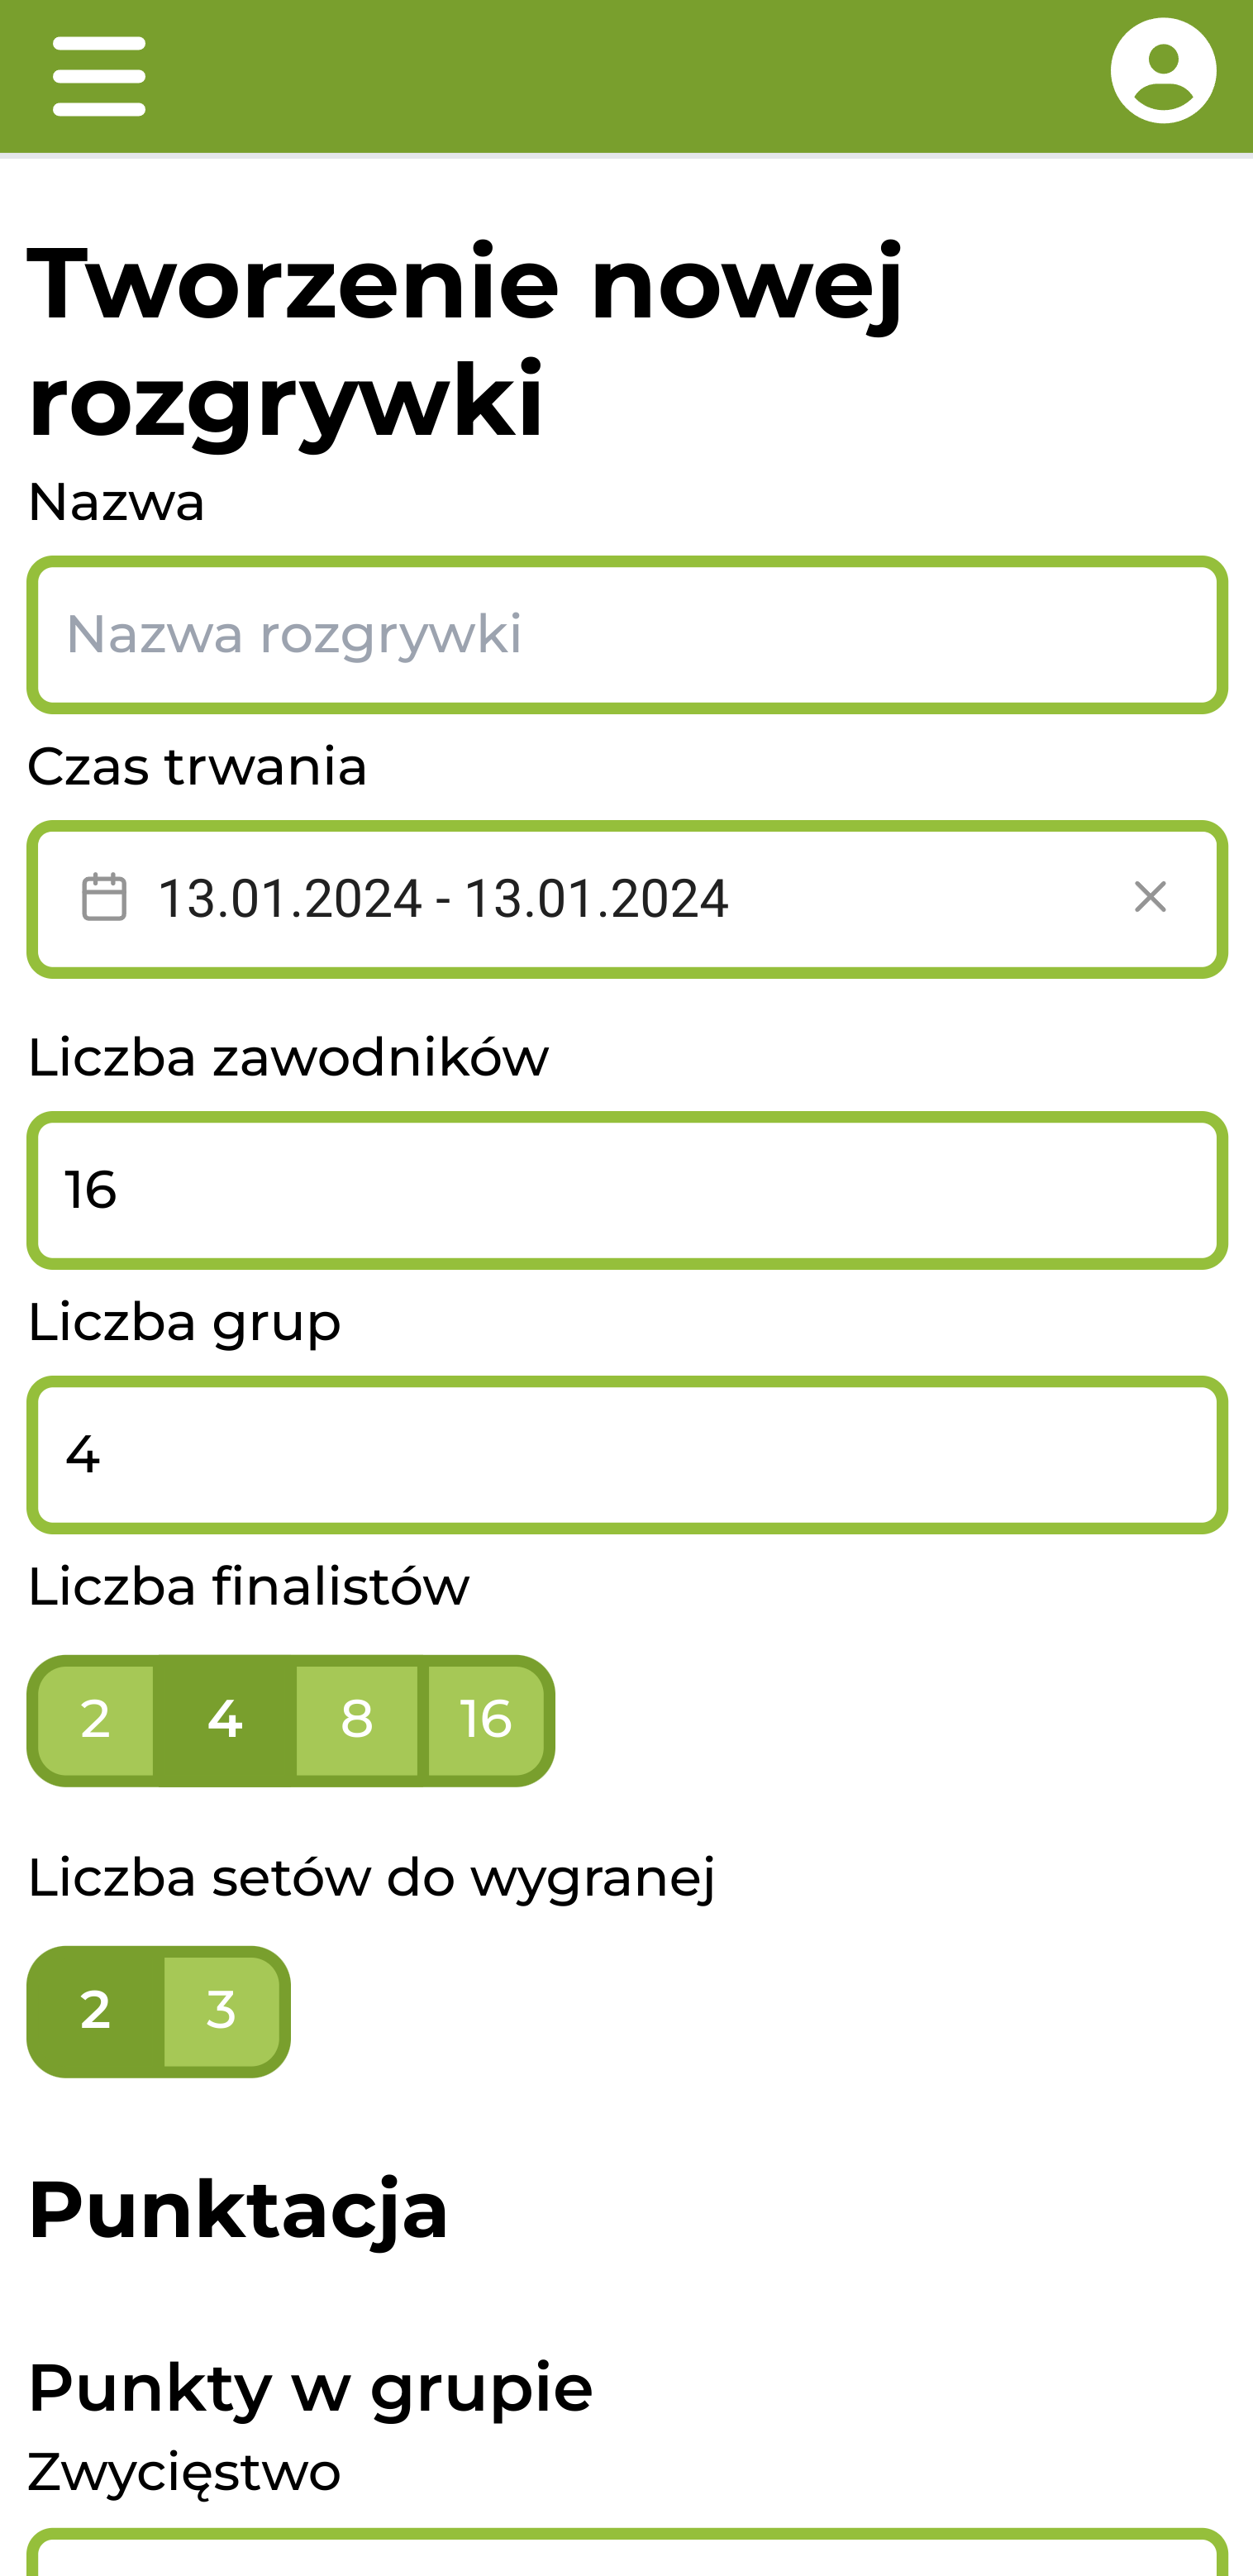
\includegraphics[width=0.22\textwidth,valign=t]{assets/interfejs/rozgrywki_utworz_mobile.png}
        \vphantom{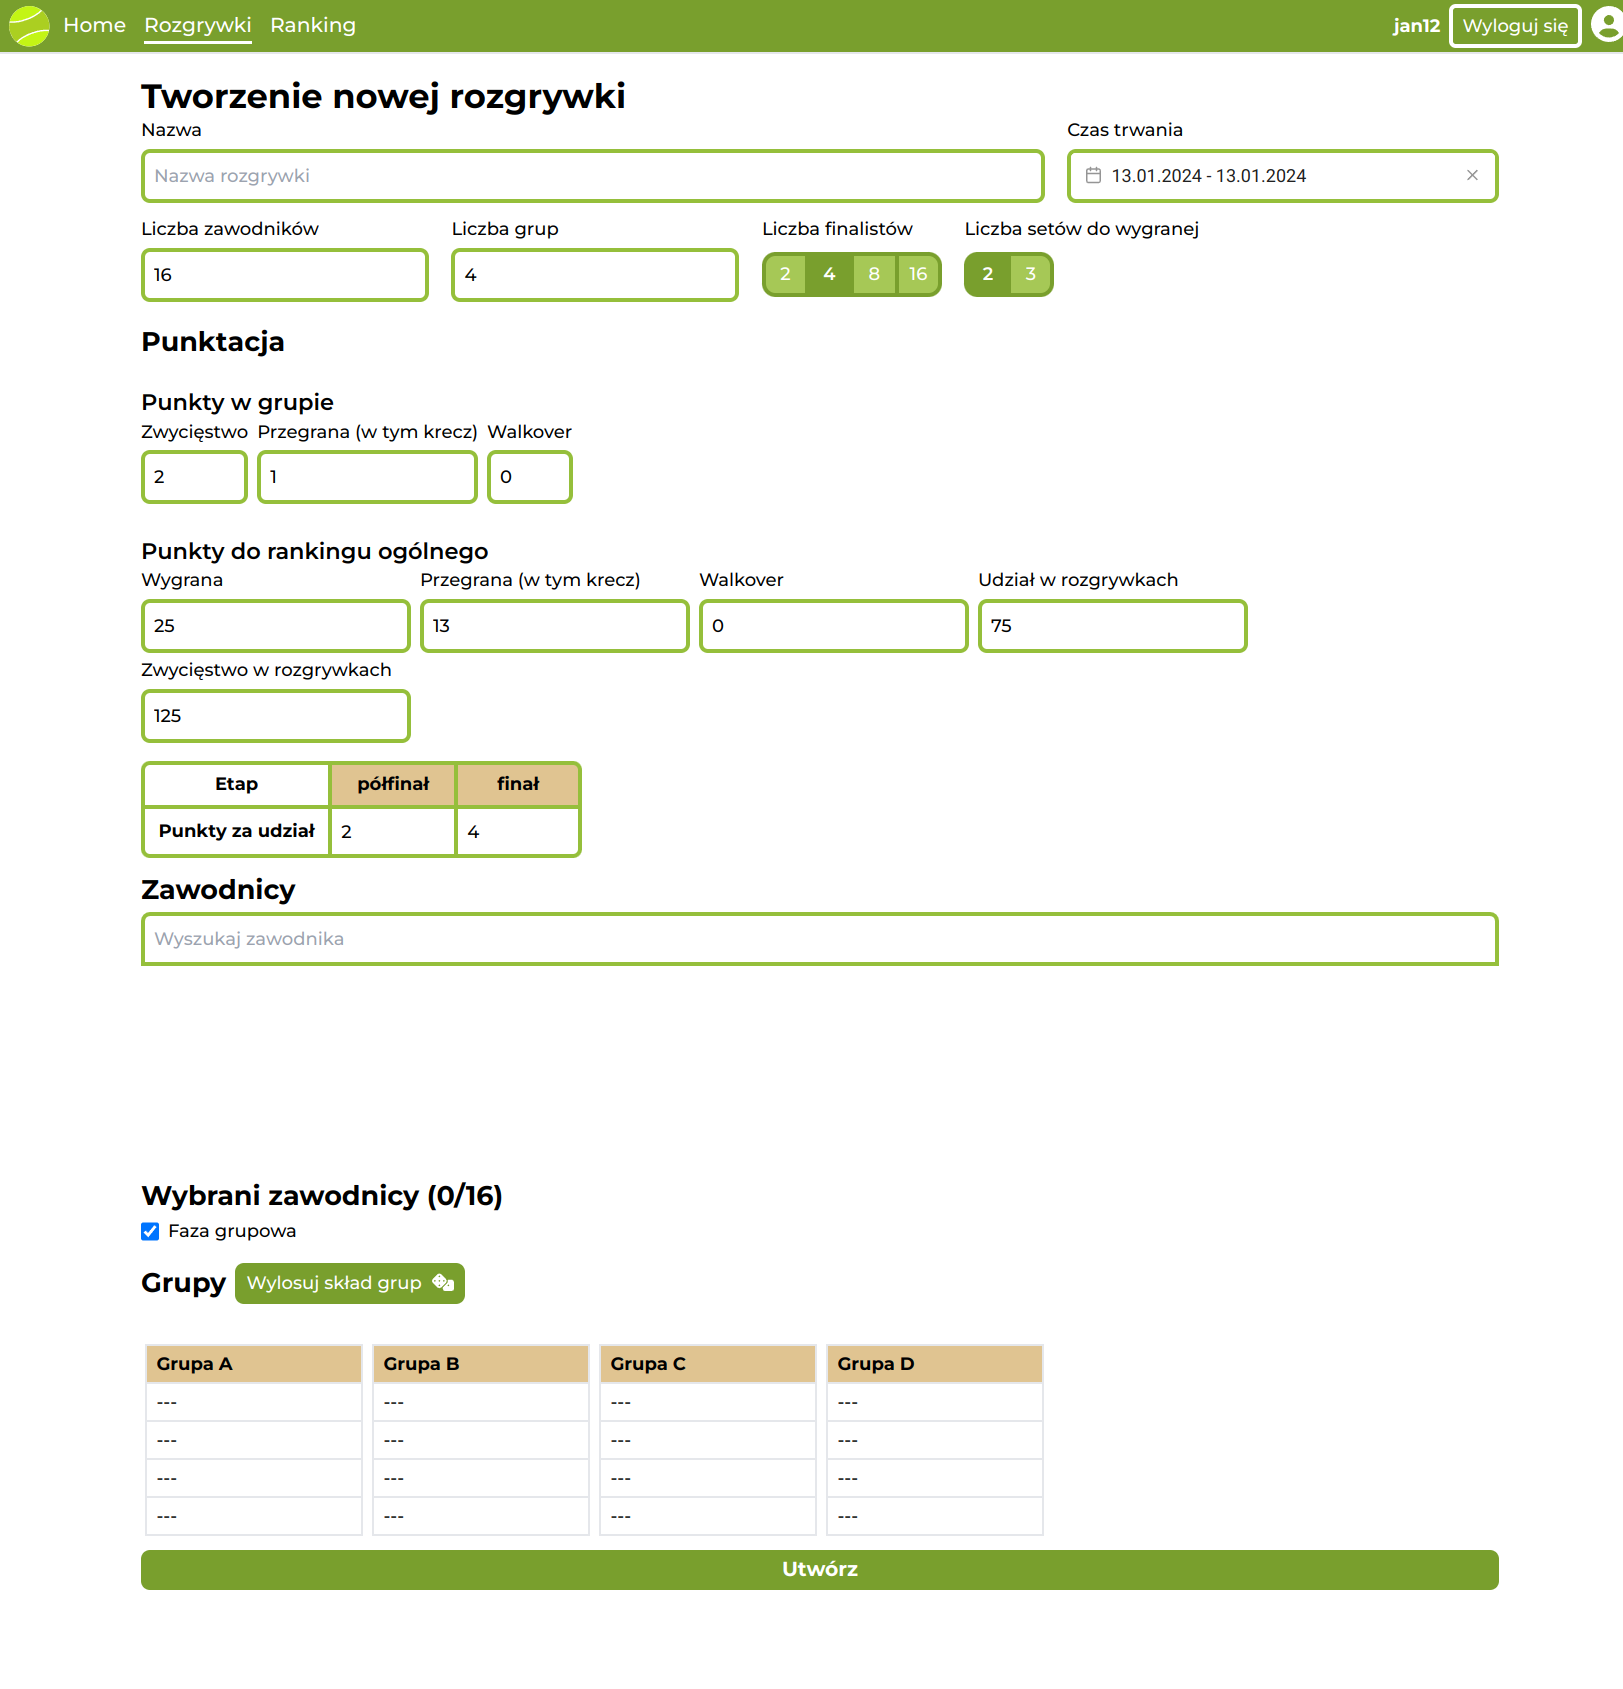
\includegraphics[width=0.72\textwidth,valign=t]{assets/interfejs/rozgrywki_utworz_desktop.png}}
    }
    \caption{Widok tworzenia rozgrywki}
    \label{fig:view_create_tournament}
\end{figure}

\newpage
\subsection{Widok rozgrywki}
U góry widoku rozgrywki~(\ref{fig:view_torunament1}) pokazane są podstawowe dane o rozgrywce i uczestnikach.
W tym miejscu użytkownik może zdobyć dane kontaktowe innych uczestników.
Następnie znajduje się tabela z aktualną sytuacją w grupie, gdzie użytkownik może znaleźć informację o sytuacji w grupach.
Dalej~(\ref{fig:view_torunament2}) znajduje się tabela pokazująca wyniki konkretnych meczów w danej grupie, klikając na dany mecz można go edytować.
Na końcu znajduje się drabinka fazy pucharowej, wraz z ikoną edycji do wprowadzania wyników.
\begin{figure}[H]
    \centering
    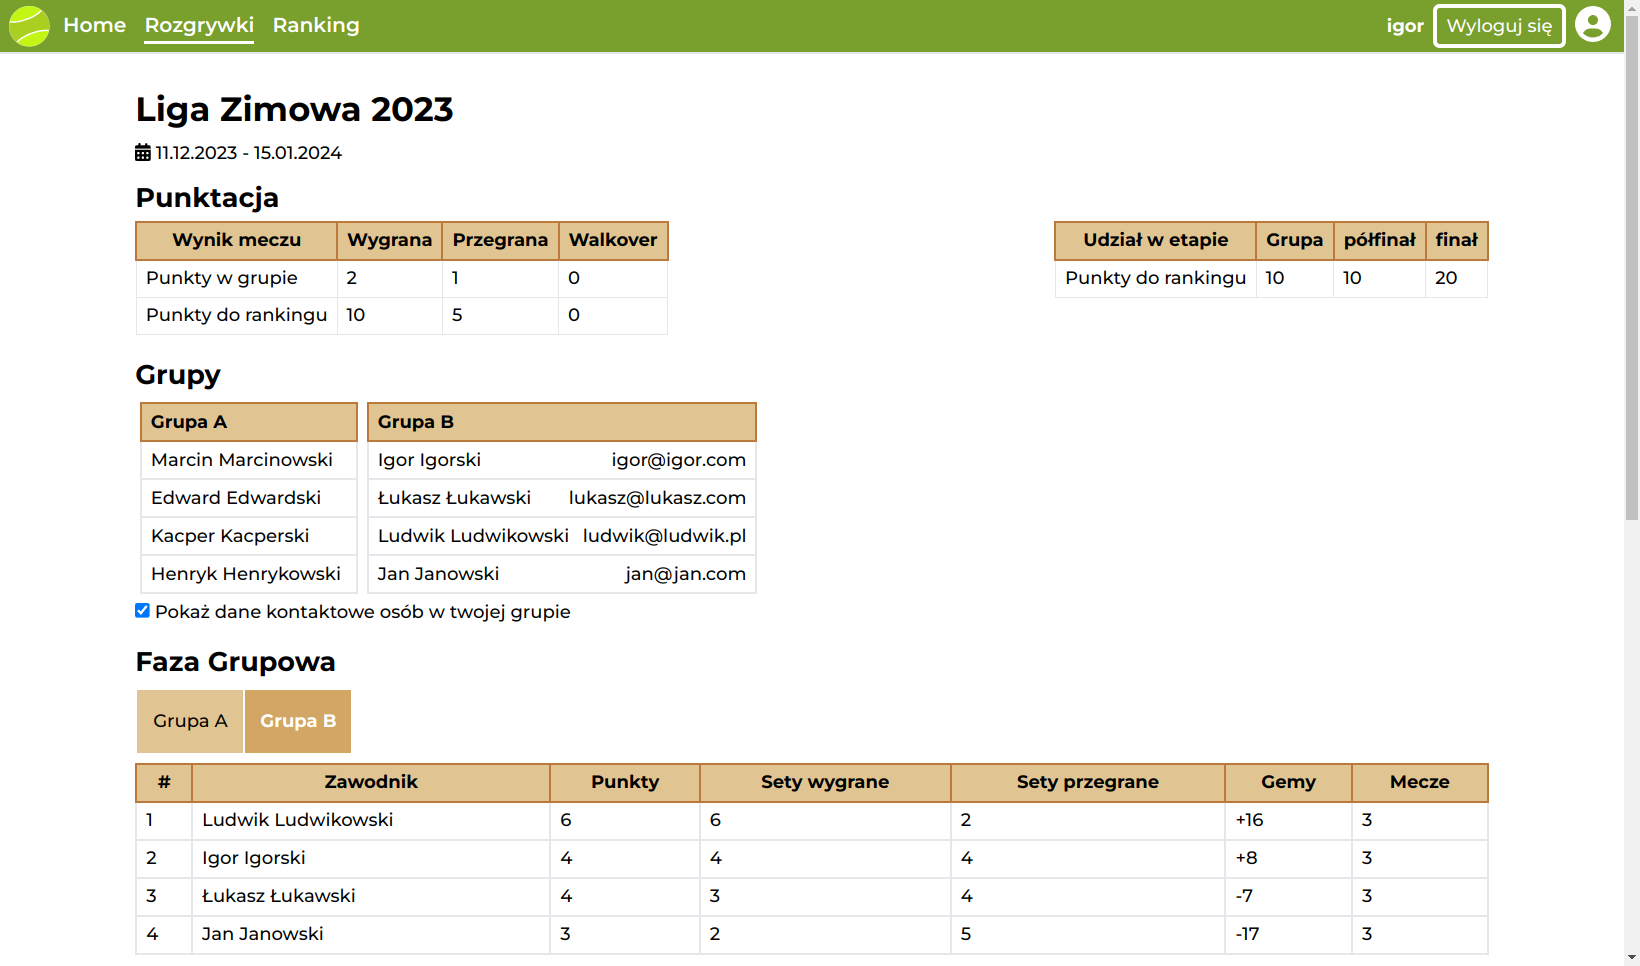
\includegraphics[width=0.72\textwidth,valign=t]{assets/interfejs/rozgrywka_desktop.png}
    \caption{Pierwsza część widoku rozgrywki}
    \label{fig:view_torunament1}
\end{figure}
\begin{figure}[H]
    \centering
    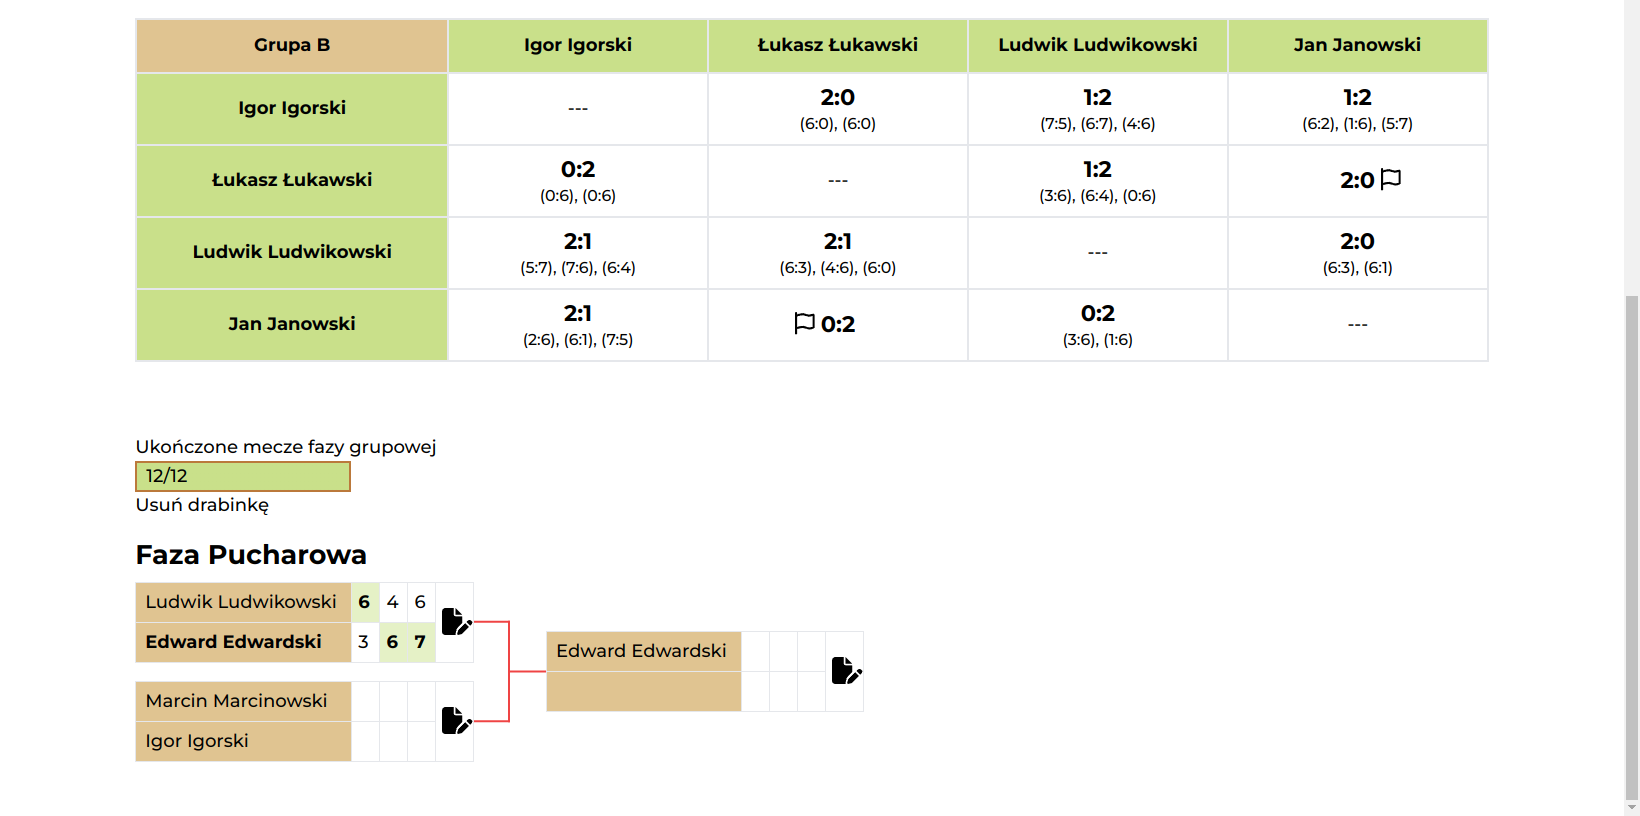
\includegraphics[width=0.72\textwidth,valign=t]{assets/interfejs/rozgrywka_desktop2.png}
    \caption{Druga część widoku rozgrywki}
    \label{fig:view_torunament2}
\end{figure}

\subsection{Widok edycji wyniku meczu}
Wynik meczu może wprowadzić\slash edytować organizator rozgrywki lub jego uczestnicy używając widoku edycji meczu~(\ref{fig:view_match_edit}).
Aplikacja weryfikuje, czy wynik jest poprawny i zaznacza na czerwono błędy. Z prawej strony wyniku
użytkownik może wybrać, jak zakończył się mecz, zgodnie z legendą, która znajduje się po niżej.
Następnie użytkownik może zapisać zmiany klikając ikonę dyskietki.

\begin{figure}[H]
    \centering
    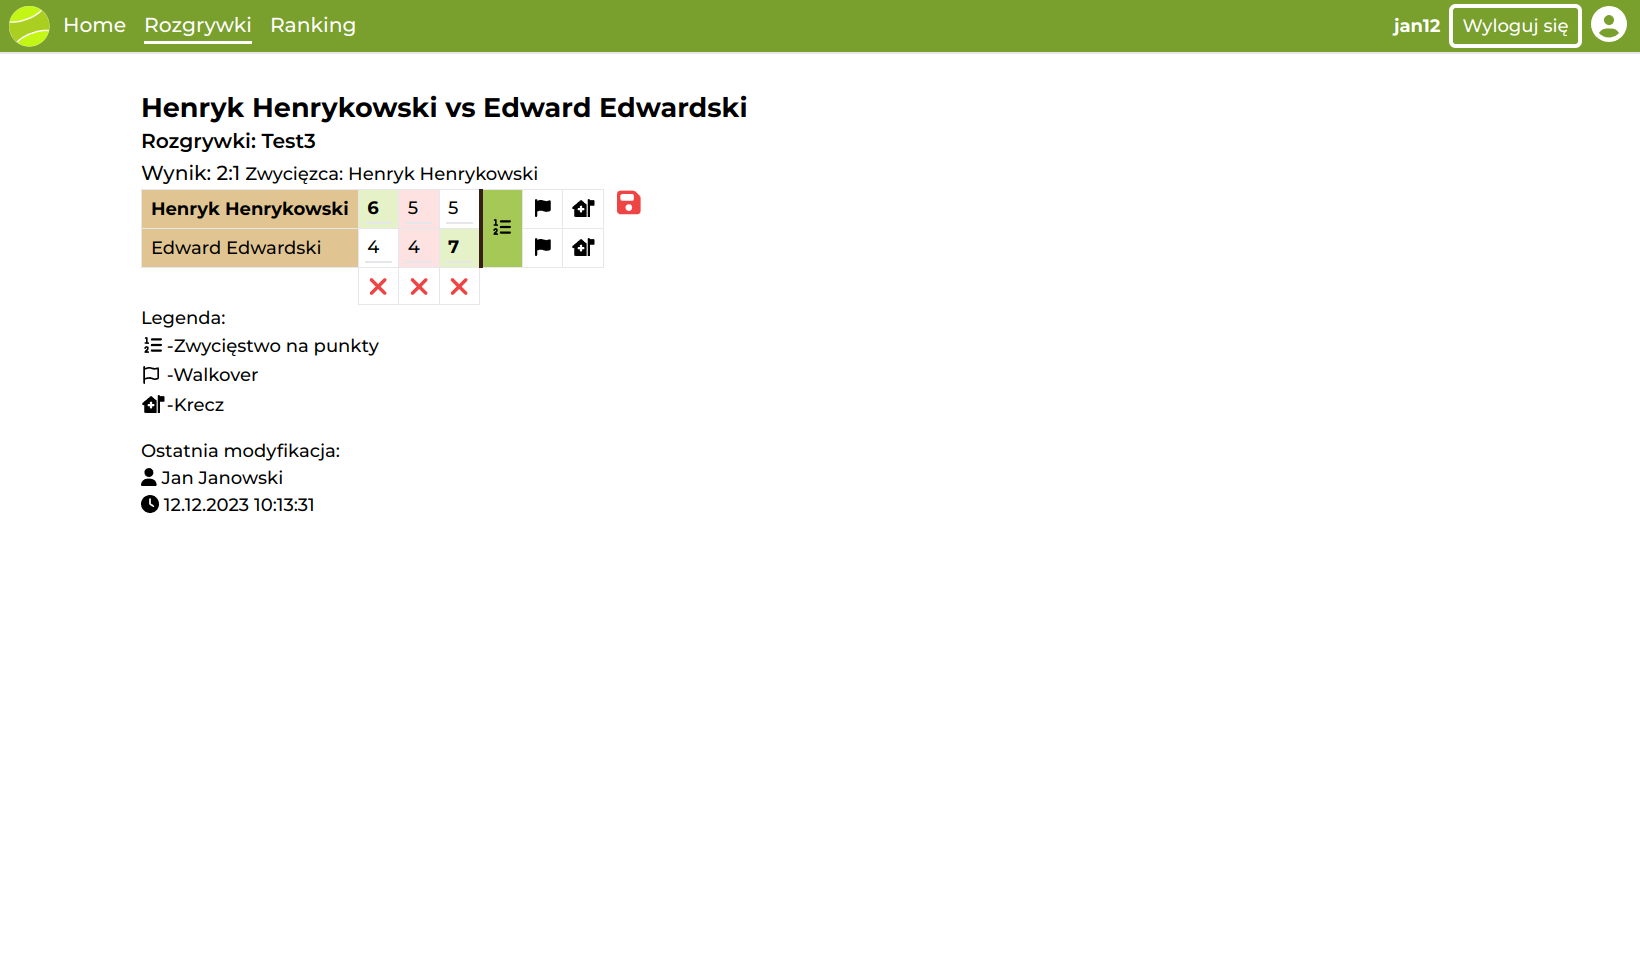
\includegraphics[width=0.72\textwidth,valign=t]{assets/interfejs/mecz_desktop.png}
    \caption{Widok edycji wyniku meczu}
    \label{fig:view_match_edit}
\end{figure}

\subsection{Weryfikacja wejścia}
Opisane w tej sekcji widoki zawierają wiele pól wprowadzania, które pozwalają na wpisywanie danych.
Nie można zakładać, że użytkownik zawsze wpisze wszystkie dane poprawnie.
W związku z tym wszystkie pola, które akceptują dane użytkownika są weryfikowane.
W przypadku wykrycia błędu aplikacja wyświetla odpowiedni komunikat~(\ref{fig:input_verification}).
\begin{figure}[H]
    \centering
    
\includegraphics[width=0.72\textwidth,valign=t]{assets/interfejs/weryfikacja_wejscia.png}
    \caption{Weryfikacja liczby zawodników i graczy w~widoku tworzenia rozgrywki}
    \label{fig:input_verification}
\end{figure}

\subsection{Wyświetlanie informacji o błędach}
Gdy wystąpi wyjątek podczas komunikacji z backendem i zostanie on przechwycony wyświetlany zostanie odpowiedni komunikat~(\ref{fig:error_mesage}).
\begin{figure}[H]
    \centering
    
\includegraphics[width=\textwidth,valign=t]{assets/interfejs/rozgrywki_error.png}
    \caption{Komunikat wyświetlany, gdy błąd został przechwycony}
    \label{fig:error_mesage}
\end{figure}

\section{Porównanie z innymi znanymi rozwiązaniami}
Aplikacja webowa rozgrywkitenisa.pl została porównana z innymi podobnymi rozwiązaniami.
Porównane zostały implementowane funkcjonalności, interfejs użytkownika oraz szybkość działania.

\subsection{Witryna playinga.com}
\texttt{Playinga.com}~\cite{Playinga} pozwala na tworzenie turniejów różnych rozgrywek sportowych~(\ref{fig:playinga_creating_tournament}).
Aplikacja ta jest darmowa i udostępnia część funkcjonalności po wykupieniu płatnej subskrypcji~(\ref{fig:playinga_paid_version}).
Przykładowo darmowa wersja nie obejmuje wpisywania wyników przez zawodników.

\begin{figure}[H]
    \centering
    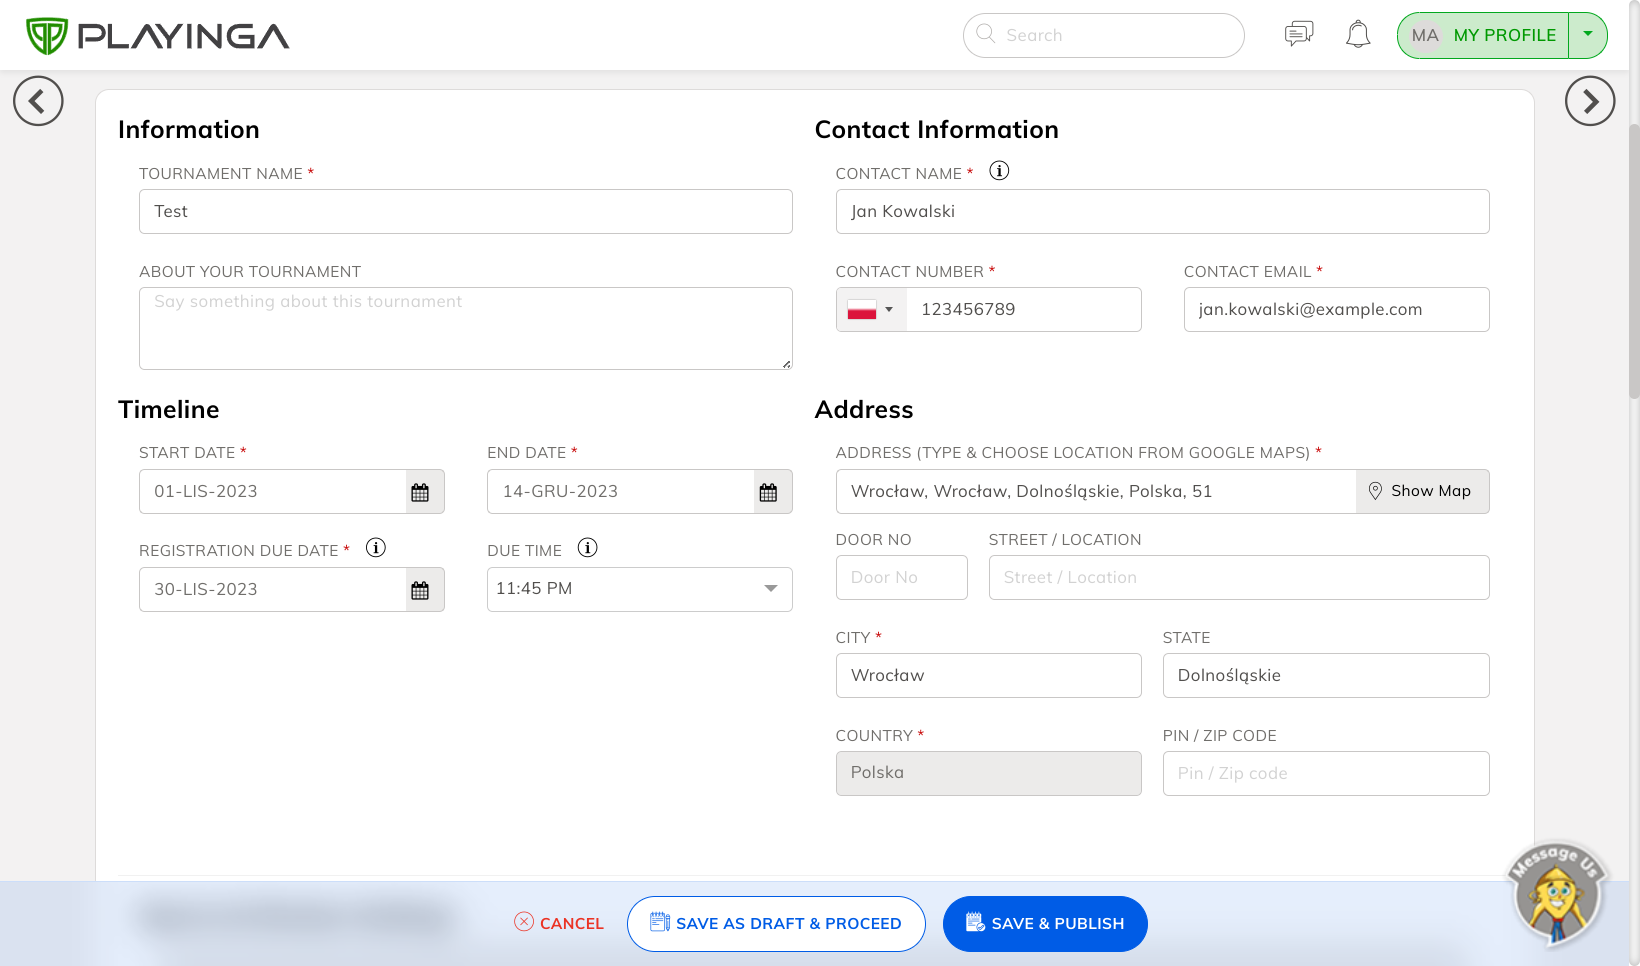
\includegraphics[width=0.72\textwidth,valign=t]{assets/alt_rozw/playinga_tworzenie.png}
    \caption{Widok tworzenia rozgrywki playinga.com}
    \label{fig:playinga_creating_tournament}
\end{figure}
\begin{figure}[H]
    \centering
    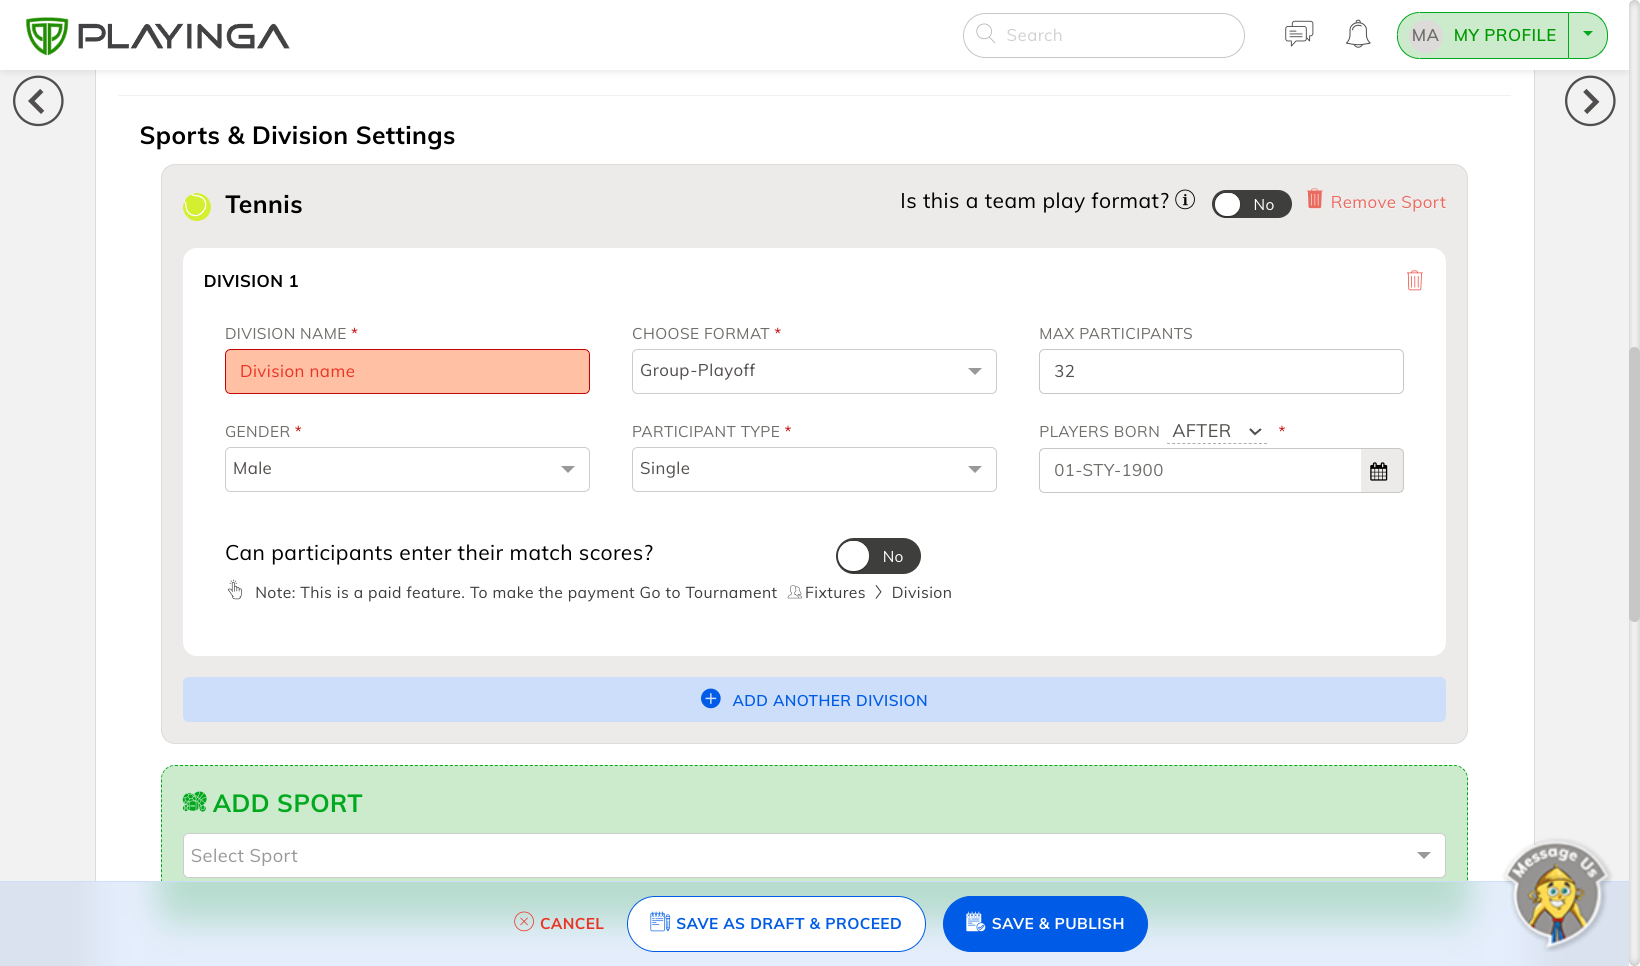
\includegraphics[width=0.72\textwidth,valign=t]{assets/alt_rozw/playinga_tworzenie2.png}
    \caption{Wpisywanie wyników przez zawodników nie jest dostępne w podstawowej wersji aplikacji}
    \label{fig:playinga_paid_version}
\end{figure}
\texttt{Playinga.com} wygląda estetycznie, a interfejs użytkownika jest responsywny. Aplikacja jest bardzo rozbudowana i umożliwia organizację turniejów z innych dziedzin sportu.
W płatnej wersji oferowane funkcjonalności pokrywają wszystkie funkcjonalności aplikacji, która jest tematem tej pracy.
\par
Jednakże \texttt{playinga.com} posiada też wady.
Po pierwsze witryna działa bardzo powoli.
Podczas testowania witryny i kliknięciu przycisku tworzącego rozgrywkę pojawiła się ikona ładowania i przez kilka minut nic się nie działo.
Jedynym rozwiązaniem tego było odświeżenie strony i ponowne uzupełnienie wszystkich danych.
Dodatkowo aplikacja zawiera niepotrzebne przekierowania.
Przykładowo zalogowany użytkownik otwierając panel użytkownika przekierowywany jest na stronę główną, a następnie z powrotem do panelu użytkownika.
Wpływa to negatywnie na wrażenia użytkownika korzystającego z aplikacji.
Kolejne problemy zauważyłem po wpisaniu danych zawodnika i kliknięciu przycisku dodaj.
Czas odpowiedzi wynosił od 5 do 10 sekund. Trzeba jednak wziąć pod uwagę, że \texttt{playinga.com} posiada nieporównywalnie więcej danych i turniejów dodanych przez wielu użytkowników.
W celu miarodajnego porównania czasu ładowania, należałoby zapełnić aplikację \texttt{rozgrywkitenisa.pl} podobną ilością danych.
Ostatnim problemem jest brak obsługi języka polskiego. Ogranicza to dostępność aplikacji dla polskojęzycznych użytkowników.
\subsection{Witryna paleta.wroclaw.pl}
\texttt{Paleta.wroclaw.pl}~\cite{PaletaWroclaw} to aplikacja webowa wrocławskiego Klubu Sportowego PALETA.
Użytkownicy internetu nienależący do klubu mogą tylko przeglądać aplikację~(\ref{fig:paleta_match_results},~\ref{fig:paleta_table_results}).
Podobnie jak w aplikacji będącej tematem pracy istnieje możliwość tworzenia rozgrywek i dodawania wyników meczów.
Niestety nie ma możliwości sprawdzenia, czy zawodnicy są uprawnieni do samodzielnego raportowania wyników spotkań.
Interfejs użytkownika jest przejrzysty, a czas reakcji strony jest wystarczająco mały, aby nie sprawiać problemu podczas przeglądania strony.
\begin{figure}[H]
    \centering
    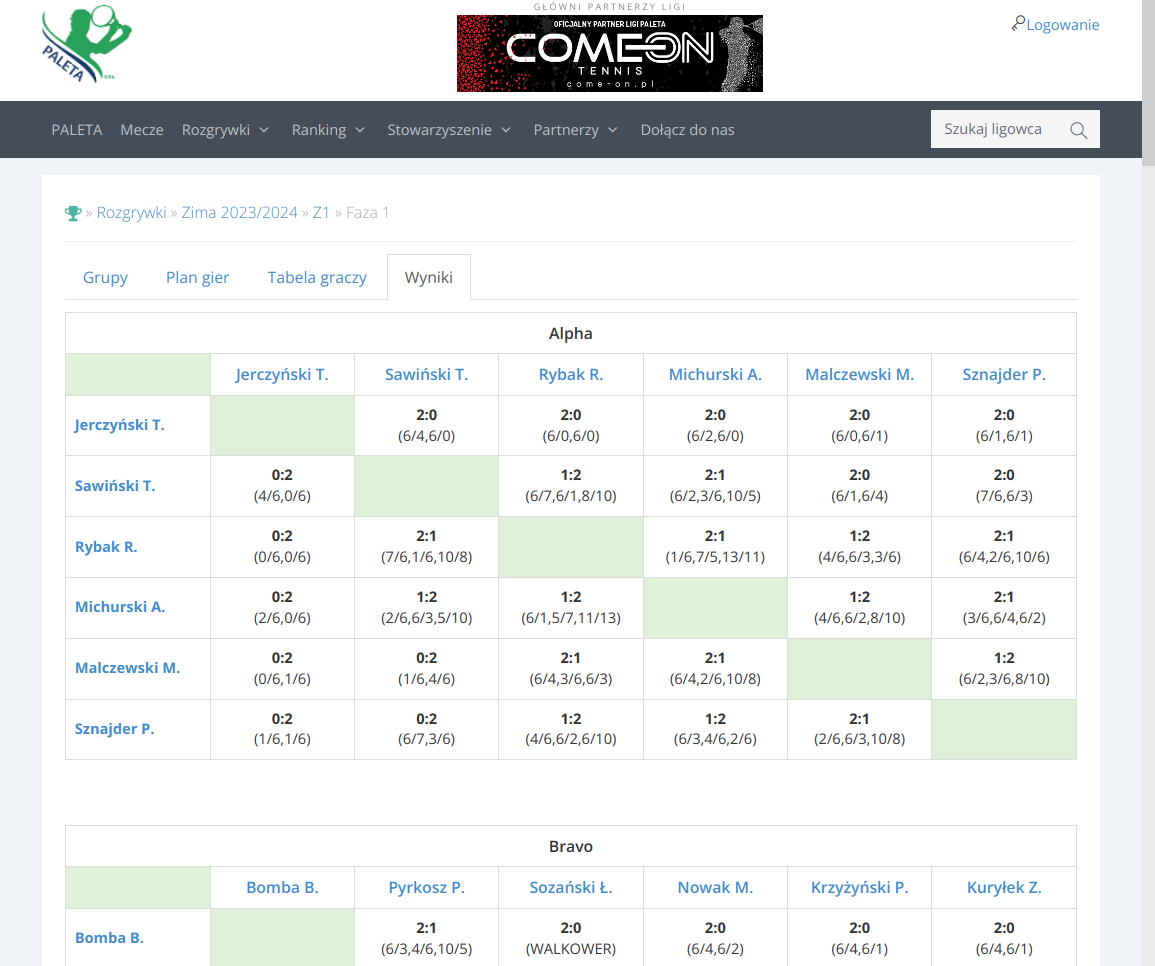
\includegraphics[width=0.72\textwidth,valign=t]{assets/alt_rozw/paleta_wyniki.png}
    \caption{Tabela wyników spotkań w witrynie paleta.wroclaw.pl}
    \label{fig:paleta_match_results}
\end{figure}
\begin{figure}[H]
    \centering
    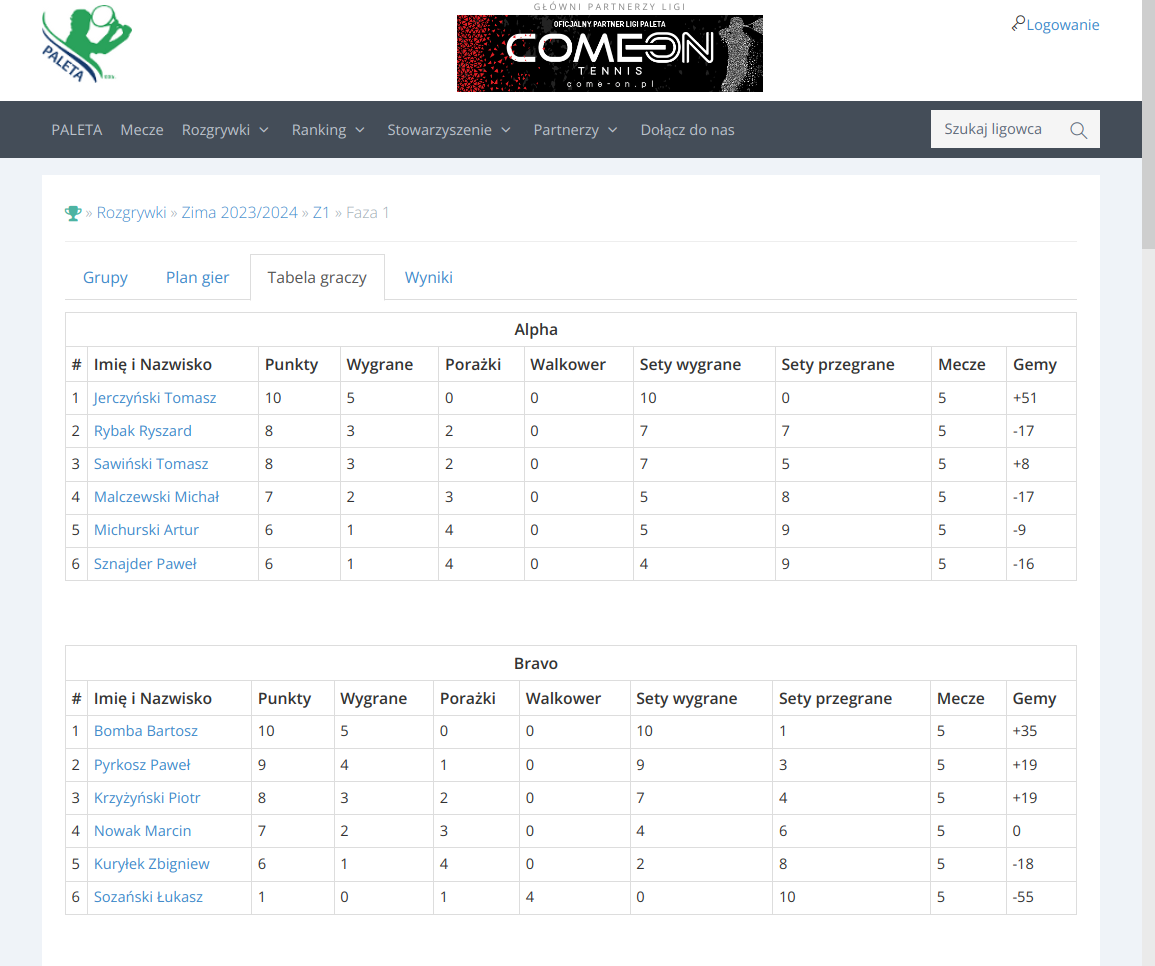
\includegraphics[width=0.72\textwidth,valign=t]{assets/alt_rozw/paleta_tabela.png}
    \caption{Tabela wyników w grupie w witrynie paleta.wroclaw.pl}
    \label{fig:paleta_table_results}
\end{figure}

\subsection{Porównanie czasu ładowania strony}
W celu porównania czasu ładowania czasu ładowania aplikacji webowej będącej tematem tej pracy z innymi rozwiązaniami, użyłem narzędzia Lighthouse.
Jest to narzędzie developerskie wbudowane w przeglądarki internetowe oparte na Chromium.
Testy zostały przeprowadzone w przeglądarce Brave w wersji 1.16.116, na laptopie z systemem operacyjnym Linux.
Laptop był wyposażony w procesor Intel i7-10750H i kartę graficzną NVIDIA GeForce RTX 2060 Mobile.
Test polegał na załadowaniu strony z listą rozgrywek. Wyniki testu są przedstawione w tabeli~\ref{tab:lighthouse_test_results}.
\begin{figure}[H]
    \centering
    \begin{tabular}{|p{3.9cm}|c|c|c|}
        \hline
                                        & rozgrywkitenisa.pl & playinga.com & paleta.wroclaw.pl \\\hline
        First Contentful Paint          & 0.6 s              & 0.6 s        & 0.7 s             \\\hline
        Largest Contentful \mbox{Paint} & 0.6 s              & 1.6 s        & 0.8 s             \\\hline
        Total Blocking Time             & 0 ms               & 470 ms       & 0 ms              \\\hline
        Cumulative Layout Shift         & 0.001              & 0.579        & 0                 \\\hline
        Speed Index                     & 0.6 s              & 2.5 s        & 0.8 s             \\\hline
    \end{tabular}
    \captionof{table}{Porównaniee metryk zmierzonych przez Lighthouse (dla każdej im mniej tym lepiej). Aplikacja będąca tematem pracy znajduje się pod adresem \texttt{rozgrywkitenisa.pl}}
    \label{tab:lighthouse_test_results}
\end{figure}
Czas ładowania strony \texttt{rozgrywkitenisa.pl} jest porównywalny z czasem ładowania strony \texttt{paleta.wroclaw.pl}.
Natomiast czas ładowania \texttt{playinga.com} jest znacznie dłuższy.
Takie same wnioski wysunąłem przeglądając wyżej wymienione strony.
Jednakże, moim zdaniem należy wziąć pod uwagę także inne aspekty działania, takie jak czas reakcji po kliknięciu.
Wtedy różnica w szybkości pomiędzy \texttt{playinga.com}, a pozostałymi witrynami jest znacznie większa.
\subsection{Podsumowanie porównania}
Aplikacja webowa będąca tematem pracy oferuje interfejs użytkownika o podobnej przejrzystości w porównaniu do alternatywnych rozwiązań.
Rozwiązania obecne na rynku oferują więcej funkcjonalności, ale duża część z nich wymaga wykupienia płatnej subskrypcji lub jest niedostępna dla zwykłych użytkowników.
Szybkość działania aplikacji webowej opisywanej w tej pracy jest porównywalna, a nawet lepsza od rozwiązań obecnych na rynku.
Może wynikać to z faktu, że baza danych witryny \texttt{rozgrywkitenisa.pl} zawiera tylko kilka rozgrywek.

\section{Instalacja}
\noindent
Repozytorium aplikacji i całej pracy znajduje się pod adresem:
\begin{center}
    \url{https://github.com/marwar22/praca-inzynierska}
\end{center}
\noindent
Aplikacja została przygotowana do uruchomienia w dwóch środowiskach:
\begin{itemize}
    \item lokalnym - do testowania na urządzeniu użytkownika,
    \item produkcyjnym - gdy aplikacja jest publicznie dostępna.
\end{itemize}
W dalszej części sekcji znajdują się instrukcje opisujące proces instalacji.
Instrukcje dla środowiska lokalnego i produkcyjnego różnią się, różnice są oznaczone.
\subsection{Zmienne środowiskowe}
\noindent
Na początku należy utworzyć pliki zawierające zmienne środowiskowe (\texttt{.env}).

\begin{itemize}
    \item
          \begin{lstlisting}[language=bash]
    cp .env.example .env
    \end{lstlisting}

    \item
          \begin{lstlisting}[language=bash]
    cd frontend
    cp .env.example .env
    \end{lstlisting}
\end{itemize}
Pliki \texttt{.env.example} zawierają przykładowe wartości, które pozwalają na uruchomienie w środowisku lokalnym.
Można je dostosować do własnej konfiguracji.


\subsection{Instalacja zależności}
Zanim będzie można zbudować i uruchomić projekt należy zainstalować \texttt{Docker} zgodnie z instrukcjami zawartymi w oficjalnej dokumentacji.
\\
\url{https://docs.docker.com/}
\\
\url{https://docs.docker.com/engine/install/}
\\
Użytkownik musi należeć do grupy \texttt{docker}

\begin{lstlisting}[language=bash]
sudo usermod -aG docker nazwa_uzytkownika
\end{lstlisting}

\subsection{Budowanie}
\noindent
Aby zbudować projekt należy wykonać poniższe polecenie:

\begin{lstlisting}[language=bash]
# środowisko produkcyjne
docker compose build
# środowisko lokalne
docker compose -f docker-compose-localhost.yml build
\end{lstlisting}

\subsection{Uruchamianie}
\begin{lstlisting}[language=bash]
# środowisko produkcyjne
docker compose up -d
# środowisko lokalne
docker compose -f docker-compose-localhost.yml up -d
\end{lstlisting}
Flaga \texttt{-d} nie jest wymagana, uruchamia projekt w tle.

\subsection{Wyłączanie}
\begin{lstlisting}[language=bash]
docker compose down
\end{lstlisting}

\subsection{Uwagi do instalacji}
Etap budowania i uruchamiania został rozdzielony, choć nie jest to konieczne.
Można zbudować i uruchomić projekt jednym poleceniem dodając flagę \texttt{--build} do odpowiedniego polecenia uruchamiającego.

Dane aplikacji są przechowywane w folderze \texttt{data/}.
W celu oczyszczenia systemu z wszystkich kontenerów, obrazów, cache i innych plików stworzonych przez Dockera należy w wykonać poniższe polecenie~\cite{DockerPrune}.
Należy wykonywać to polecenie z rozwagą, ponieważ usuwa ono także kontenery, obrazy i pliki z innych projektów Dockera.
\begin{lstlisting}[language=bash]
docker system prune
\end{lstlisting}
Przed uruchomieniem należy upewnić się, że żaden inny proces nie używa portu 80 lub 443.
Przykładowo domyślna instalacja KDE Neon i innych dystrybucji Linuxa opartych na Ubuntu uruchamia apache2, który używa port 80.
Aby zatrzymać apache2 należy wykonać polecenie:
\begin{lstlisting}[language=bash]
sudo systemctl stop apache2
\end{lstlisting}

\chapter{Architektura aplikacji}
Opis architektury aplikacji składa się z ogólnego zarysu struktury oraz bardziej szczegółowego opisu każdej części.
\section{Struktura aplikacji}
Aplikacja została podzielona na 5 głównych części:
\begin{itemize}
    \item \textbf{frontend} - cześć aplikacji widoczna dla użytkownika
    \item \textbf{backend} - odpowiada za przekazywanie i odbieranie danych od frontendu, odczytuje i zapisuje dane do bazy danych
    \item \textbf{baza danych} - przechowuje dane aplikacji
    \item \textbf{reverse proxy} - wysyła, odbiera, przekazuje zapytania do odpowiednich części aplikacji
    \item \textbf{narzędzie do odnawiania certyfikatów SSL/TLS} - automatyzuje proces odnawiania certyfikatów SSL/TLS
\end{itemize}
Każda część aplikacji jest opisana w następnej sekcji.

\section{Kontenery Dockera}
W celu utrzymania dobrej współpracy pomiędzy wszystkimi elementami aplikacji zdecydowałem się użyć Dockera\cite{Docker}.
Każda z 5 części aplikacji jest opakowywana w osobny kontener, czyli lekką maszynę wirtualną, która zawiera tylko potrzebne do jej działania zależności.
Konfiguracja całego środowiska znajduje się w pliku \texttt{docker-compose.yml}. Najważniejsze elementy zostały pokazane na rysunku \ref{fig:docker_containers_environment}.

\begin{figure}[H]
    \centering
    \includegraphics[width=\textwidth]{assets/środowisko_dockera.png}
    \caption{Struktura kontenerów Dockera}
    \label{fig:docker_containers_environment}
\end{figure}

\subsection{Reverse Proxy - Nginx}
Nginx\cite{Nginx} działa jako Reverse Proxy i jest odpowiedzialny za przekierowywanie zapytań http i https do odpowiednich części aplikacji.
W folderze \texttt{nginx/config/} znajdują się 3 pliki konfiguracyjne. Podczas działania aplikacji używany jest dokładnie jeden z nich.

\begin{itemize}
    \item \texttt{nginx\_init\_ssl\_certificate.conf} jest używany podczas pierwszego uruchomienia w środowisku produkcyjnym, obsługuje tylko zapytania http i pozwala kontenerowi Certbot(\ref{subsec:Certbot}) na pobranie certyfikatu SSL/TLS. Jest potrzebny, ponieważ nie jest możliwe obsługiwanie zapytań https bez poprawnego certyfikatu SSL/TLS.
    \item \texttt{nginx.conf} jest używany w środowisku produkcyjnym. Definiuje przekierowywanie zapytań do odpowiednich kontenerów. W tej konfiguracji nieszyfrowana komunikacja za pomocą http jest przekierowywana do szyfrowanej komunikacji za pomocą https.
    \item \texttt{nginx\_localhost.conf} jest używany w środowisku lokalnym.
\end{itemize}
\begin{figure}[H]
    \centering
    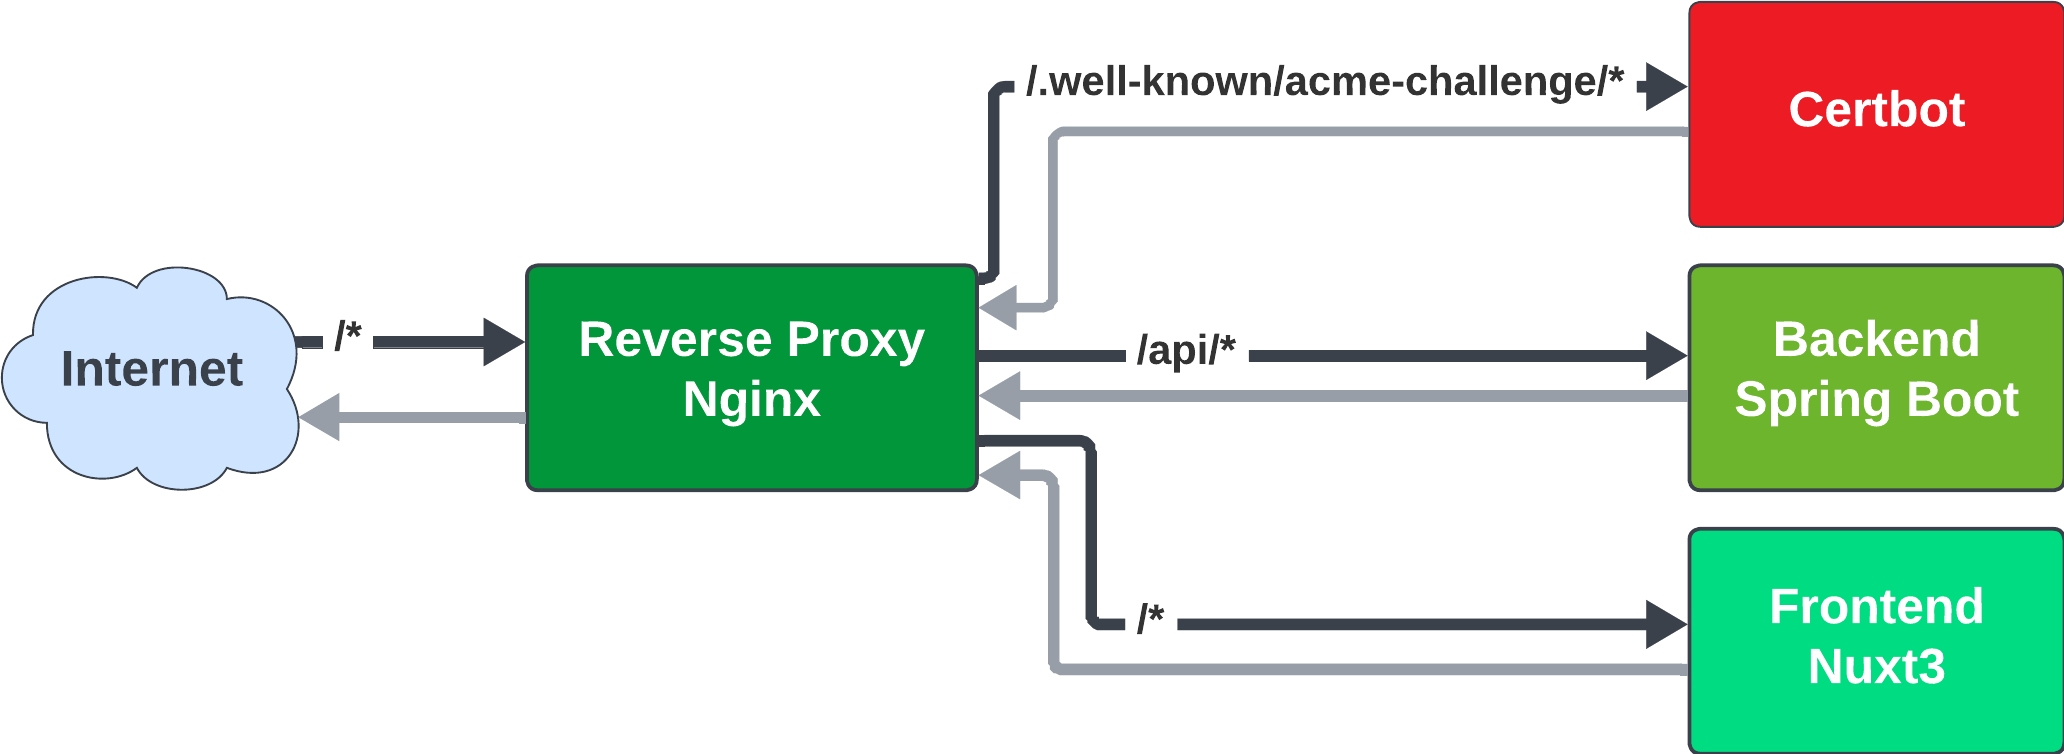
\includegraphics[width=\textwidth]{assets/przepływ_zapytań_http.png}
    \caption{Przepływ zapytań https zdefiniowanych w pliku \texttt{nginx.conf}}
    \label{fig:https_requests_flow}
\end{figure}
Na rysunku \ref{fig:https_requests_flow} pokazano schemat przepływu zapytań https dla pliku \texttt{nginx.conf}.
W przypadku zapytania http reverse proxy nie przekazuje zapytania do kolejnego kontenera, a odpowiada klientowi od razu przekierowaniem do https. Dla zapytań https zdefiniowane są następujące reguły:
\begin{enumerate}
    \item Jeżeli url zaczyna się od \texttt{/.well-known/acme-challenge/} przekaż zapytanie do kontenera Certbot.
    \item Jeżeli url zaczyna się od \texttt{/api} przekaż zapytanie do kontenera backend.
    \item W przeciwnym przypadku przekaż zapytanie do kontenera frontend.
\end{enumerate}
Wszystkie odpowiedzi na zapytania przekazywane są do reverse proxy, a reverse proxy przekazuje je dalej do nadawcy zapytania.

\subsection{Frontend - Nuxt3, Vue.js}
Frontend został napisany we frameworku Nuxt3~\cite{Nuxt3}, który oparty jest na Vue.js.
Użyłem języka TypeScript, ponieważ wprowadza on statyczne typowanie.
TypeScript w porównaniu do JavaScriptu ułatwił pisanie kodu, dzięki lepszym podpowiedziom środowiska programistycznego oraz pozwolił zapobiegać błędom, szybciej ostrzegając o problemach podczas kompilacji.
Do utrzymania jednolitego formatowania kodu źródłowego użyłem narzędzia Prettier~\cite{Prettier}.
Kod źródłowy frontendu znajduje się w folderze \texttt{frontend/}. W projekcie struktura plików frontendu oparta jest na
standardach zdefiniowanych w dokumentacji Nuxt3.
\begin{figure}[H]
    \dirtree{%
        .1 frontend.
        .2 components.
        .2 composables.
        .2 pages.
        .2 plugins.
        .2 public.
        .2 middleware.
        .2 types.
        .2 utils.
    }
    \caption{Zarys struktury plików}
\end{figure}

\noindent
Zawartość tych folderów jest następująca:
\begin{itemize}
    \item \texttt{components/} zawiera elementy interfejsu użytkownika (np. tabela wyników, element tablicy wyników, drabinka turniejowa)
    \item \texttt{composables/} zawiera elementy logiki, które posiadają swój stan i są używane w wielu miejscach. Moja aplikacja definiuje \texttt{AuthStatus}, który jest odpowiedzialny za przechowywanie informacji o tym, czy użytkownik jest zalogowany, czy nie.
    \item \texttt{pages/} struktura adresów url odpowiada plikom w tym folderze\\(np. \texttt{rozgrywkitenisa.pl/rozgrywki/123} $\longrightarrow$ \texttt{pages/rozgrywki/[id].vue})
    \item \texttt{plugins/} zawiera konfigurację dwóch pluginów (FontAwesome~\cite{FontAwesome} (dostarcza ikony aplikacji), VueDatePicker~\cite{VueDatePicker} (Dostarcza narzędzie do wybierania daty)
    \item \texttt{public/} zawiera statyczne pliki, które nie są zmieniane podczas kompilacji i~są przekazywane jako niezmienione klientowi
    \item \texttt{middleware/} zawiera middleware, które odpowiedzialne są za modyfikowanie zapytań przed przekazaniem ich dalej. Moja aplikacja używa tylko 1 middleware \texttt{logged.in.ts}, który przekierowuje niezalogowanych użytkowników do strony logowania
    \item \texttt{types/} zawiera pliki definiujące typy języka TypeScript
    \item \texttt{utils/} zawiera funkcje i stałe używane w co najmniej 2 plikach aplikacji
\end{itemize}
Oprócz wyżej wymienionych technologii zastosowałem bibliotekę TailwindCSS~\cite{TailwindCSS} do stylizacji aplikacji.
W pliku \texttt{tailwind.config.js} znajduje się konfiguracja tej biblioteki, wraz z dedykowaną dla tego projektu paletą kolorów.
Wielokrotnie używałem prefiksów dla stylów oferowanych przez TailwindCSS, które aktywują/dezaktywują dany styl w zależności od wielkości ekranu.
Dzięki temu aplikacja jest responsywna i dostosowana zarówno do komputerów jak i urządzeń mobilnych.


\subsection{Backend - Spring Boot}
Backend napisałem używając frameworka Spring Boot. Do zarządzania zależnościami i do automatyzacji budowania użyłem narzędzia Maven.
\\Kod backendu został podzielony na warstwy:
\begin{itemize}
    \item \textbf{kontrolery} - odpowiedzialne za przetworzenie parametrów żądania, wysłanie odpowiedzi
    \item \textbf{serwisy} - odpowiedzialne za logikę biznesową backendu
    \item \textbf{repozytoria} - odpowiedzialne za komunikację z bazą danych
\end{itemize}
Dodatkowo każdy obiekt przechowywany w bazie danych posiada klasy odpowiedzialne za ich działanie:
\begin{itemize}
    \item \textbf{encje} - definiują pola, cechy obiektu przechowywanego w bazie danych
    \item \textbf{obiekty} transferu danych (DTO) - definiują obiekty przesyłane z serwera lub do serwera
    \item \textbf{maper} - klasy służące do konwertowania obiektów między encjami, a obiektami transferu danych
\end{itemize}
Przykładowo dla obiektu odpowiedzialnego za rozgrywkę (\texttt{Tournament}) zdefiniowane są następujące klasy:
\begin{itemize}
    \item \texttt{TournamentController} - kontroler
    \item \texttt{TournamentMapper} - maper
    \item \texttt{TournamentRepository} - repozytorium
    \item \texttt{TournamentService} - serwis
    \item \texttt{Tournament} - encja
    \item \texttt{TournamentCreateDto} - obiekt transferu danych wysyłany przez frontend podczas żądania stworzenia rozgrywki
    \item \texttt{TournamentBasicDto} - obiekt transferu danych zawierający tylko podstawowe informacje o rozgrywce, jest używany podczas wysyłania listy wszystkich rozgrywek
\end{itemize}

\subsection{Baza danych - PostgreSQL}
Do przechowywania danych wybrałem PostgreSQL.
Zdecydowałem się wybrać tą technologię ze względu na to, że chciałem użyć relacyjnej bazy danych, która jest wydajna, niezawodna i aktywnie rozwijana. PostgreSQL spełnia wszystkie te wymagania.
\par
Konfiguracja bazy danych jest zarządzana przez backend i narzędzie Flyway~\cite{Flyway}.
W~folderze \texttt{backend/src/main/resources/db/migration} znajdują się pliki z poleceniami SQL definiujące migracje pomiędzy wersjami.
Gdy schemat bazy danych był zmieniany, dokładałem kolejny plik odpowiedzialny za migrację. Przy uruchomieniu backendu Flyway automatycznie sprawdza, czy zostały dodane jakieś pliki migracyjne.
Jeżeli tak, to dokonuje migracji.
Dzięki temu baza danych używana lokalnie oraz baza danych na serwerze w wersji produkcyjnej, utrzymują ten sam schemat bazy danych.

\subsection{Narzędzie do odnawiania certyfikatów SSL/TLS - Certbot}
Dla bezpieczeństwa użytkowników połączenie ze stroną internetową powinno być szyfrowane.
Do nawiązania szyfrowanego połączenia używane są certyfikaty SSL/TLS, które zawierają klucz publiczny i inne dane, takie jak okres ważności, dane właściciela, wystawcy.
Każdy ma możliwość wystawić własny certyfikat, ale przeglądarka będzie ufać tylko certyfikatom wydanym przez zaufane (według twórców przeglądarki) instytucje.
Świadomy użytkownik znając wystawcę certyfikatu może ręcznie dodać go do listy zaufanych certyfikatów. Takie rozwiązanie jest właściwe tylko wtedy, gdy nie chcemy powierzać generowania kluczy zewnętrznej instytucji i użytkownicy mogą potwierdzić jego prawdziwość (np. gdy wystawiamy certyfikat aplikacji webowej do użytku wewnętrznego firmy).
W związku z tym, że aplikacja webowa będąca tematem pracy będzie publicznie dostępna, generowanie certyfikatów SSL/TLS powierzyłem organizacji Let's Encrypt~\cite{LetsEncrypt}.
Let's Encrypt wystawia darmowe certyfikaty SSL/TLS oraz umożliwia automatyzację tego procesu.
Kontener Certbot oparty jest na narzędziu o tej samej nazwie~\cite{Certbot}.
Odpowiada on za automatyczne odnawianie certyfikatów poprzez wysyłanie zapytania do Let's Encrypt i odpowiadanie serwerom tej organizacji na zapytania weryfikujące - czy prośbę o~wydanie certyfikatu wysłał właściciel domeny rozgrywkitenisa.pl.

\label{subsec:Certbot}

%%%%% BIBLIOGRAFIA

\begin{thebibliography}{1}
    \bibitem{Docker} Dokumentacja Dockera \url{https://docs.docker.com/}
    \bibitem{DockerPrune} Dokumentacja polecenia docker system prune \url{https://docs.docker.com/engine/reference/commandline/system_prune/}
    \bibitem{Nginx} Dokumentacja Nginx \url{https://docs.nginx.com/}
    \bibitem{Nuxt3} Nuxt3 \url{https://nuxt.com/}
    \bibitem{Prettier} Prettier \url{https://prettier.io/}
    \bibitem{Nuxt3DocsPages} Nuxt3 - dokumentacja struktury plików w folderze pages/, \url{https://nuxt.com/docs/guide/directory-structure/pages}
    \bibitem{FontAwesome} FontAwesome \url{https://fontawesome.com/docs}
    \bibitem{VueDatePicker} VueDatePicker \url{https://vue3datepicker.com/}
    \bibitem{TailwindCSS} TailwindCSS \url{https://tailwindcss.com/}
    \bibitem{SpringBoot} SpringBoot \url{https://spring.io/projects/spring-boot/}
    \bibitem{Flyway} Flyway \url{https://flywaydb.org/}
    \bibitem{Certbot} Certbot \url{https://certbot.eff.org/}
    \bibitem{LetsEncrypt} LetsEncrypt \url{https://letsencrypt.org/pl/}
    \bibitem{PaletaWroclaw} PALETA \url{https://www.paleta.wroclaw.pl/}
    \bibitem{Playinga} Playinga \url{https://playinga.com/}
\end{thebibliography}

\end{document}